\begin{abox}
TIFR 2020
\end{abox}
\begin{questions}
\begin{minipage}{\textwidth}
	\question A three-dimension view of a solid is sketched below:\\
	\begin{figure}[H]
		\centering
		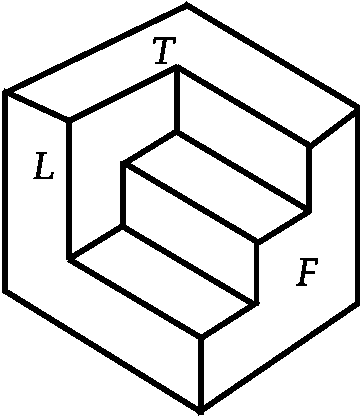
\includegraphics[height=4cm,width=4cm]{t330}
	\end{figure}
	The three projections below are each intended to show the solid from its front $(F)$, left side $(L)$ and top $(T)$, as marked in the figure. Which one is correct?
	\exyear{TIFR 2020}
\end{minipage}
\begin{tasks}(1)
	\task[\textbf{A.}] \begin{figure}[H]
		\centering
		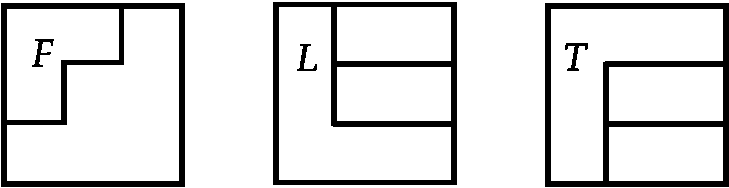
\includegraphics[height=2.5cm,width=9.5cm]{t331}
	\end{figure}
	\task[\textbf{B.}] \begin{figure}[H]
		\centering
		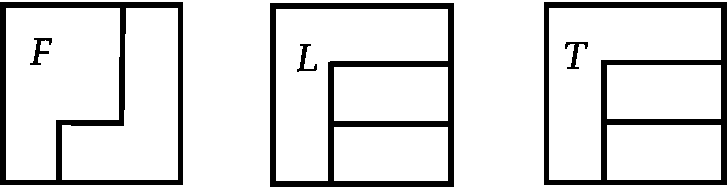
\includegraphics[height=2.5cm,width=9.5cm]{t332}
	\end{figure}
	\task[\textbf{C.}] \begin{figure}[H]
		\centering
		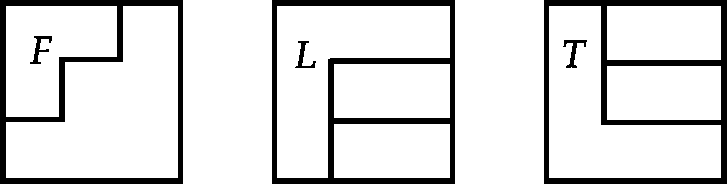
\includegraphics[height=2.5cm,width=9.5cm]{t333}
	\end{figure}
	\task[\textbf{D.}] \begin{figure}[H]
		\centering
		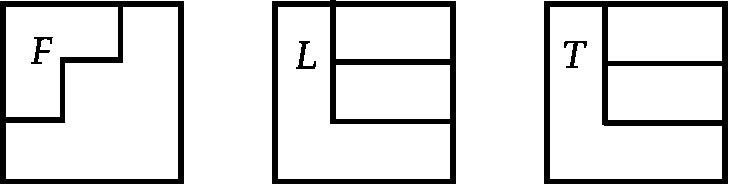
\includegraphics[height=2.5cm,width=9.5cm]{t334}
	\end{figure}
\end{tasks}
\begin{answer}
	So the correct answer is \textbf{option(A)}
\end{answer}
\begin{minipage}{\textwidth}
	\question The limit $\lim _{x \rightarrow \infty} x \log \frac{x+1}{x-1}$
	Evaluate to
	\exyear{TIFR 2020}
\end{minipage}
\begin{tasks}(4)
	\task[\textbf{A.}] 2
	\task[\textbf{B.}] 0
	\task[\textbf{C.}] $\infty$
	\task[\textbf{D.}] 1
\end{tasks}
\begin{answer}
	$\begin{aligned} x \log \frac{x+1}{x-1} &=x \log \frac{x+1 / x}{x-1 / x} \\ &=x\left[\log \left(1+\frac{1}{x}\right)-\log \left(1-\frac{1}{x}\right)\right] \\ &=x\left[\left(\frac{1}{x}-\frac{1}{2 x^{2}}+\frac{1}{3 x^{3}} \ldots\right)-\left(-\frac{1}{x}-\frac{1}{2} x^{2}-\frac{1}{3 x^{2}} \ldots\right)\right] \\ &=x\left[\frac{2}{x}+\frac{2}{3 x^{3}} \ldots\right] \\ &=\left[2+\frac{2}{3 x^{3}}+\ldots .\right] \end{aligned}$\\
	So, $\lim _{x \rightarrow \infty} x \log \frac{x+1}{x-1}=2$\\
	So the correct answer is \textbf{option(A)}
	
\end{answer}
\begin{minipage}{\textwidth}
	\question The eigenvector $e_{1}$ corresponding to the smallest eigenvalue of the matrix
	$$
	\left(\begin{array}{ccc}
	2 a^{2} & a & 0 \\
	a & 1 & a \\
	0 & a & 2 a^{2}
	\end{array}\right)
	$$
	where $a=\sqrt{\frac{3}{2}}$ is given (in terms of its transpose) by
	\exyear{TIFR 2020}
\end{minipage}
\begin{tasks}(2)
	\task[\textbf{A.}] $e_{1}^{T}=\frac{1}{2}\left(\frac{1}{\sqrt{2}}-\sqrt{3} \frac{1}{\sqrt{2}}\right)$
	\task[\textbf{B.}] $e_{1}^{T}=\frac{1}{2}\left(\sqrt{\frac{3}{2}} \quad 1 \quad \sqrt{\frac{3}{2}}\right)$
	\task[\textbf{C.}] $e_{1}^{T}=\frac{1}{\sqrt{2}}\left(\begin{array}{lll}1 & 0 & -1\end{array}\right)$
	\task[\textbf{D.}] $e_{1}^{T}=\frac{1}{\sqrt{2}}\left(\begin{array}{lll}1 & 0 & 1\end{array}\right)$
\end{tasks}
\begin{answer}
	Matrix
	$$
	\begin{aligned}
	A &=\left[\begin{array}{ccc}
	2 a^{2} & a & 0 \\
	a & 1 & a \\
	0 & a & 2 a^{2}
	\end{array}\right] \text { where } a=\sqrt{\frac{3}{2}} \\
	&=\left[\begin{array}{ccc}
	3 & \sqrt{\frac{3}{2}} & 0 \\
	\sqrt{\frac{3}{2}} & 1 & \sqrt{\frac{3}{2}} \\
	0 & \sqrt{\frac{3}{2}} & 3
	\end{array}\right] \\
	A e_{1} &=\left[\begin{array}{ccc}
	3 & \sqrt{\frac{3}{2}} & 0 \\
	\sqrt{\frac{3}{2}} & 1 & \sqrt{\frac{3}{2}} \\
	0 & \sqrt{\frac{3}{2}} & 3
	\end{array}\right]\left[\begin{array}{c}
	\frac{1}{\sqrt{2}} \\
	-\sqrt{3} \\
	\frac{1}{\sqrt{3}}
	\end{array}\right]=\left[\begin{array}{l}
	0 \\
	0 \\
	0
	\end{array}\right]
	\end{aligned}
	$$\\
	So, $e_{1}$ is eigenvector corresponding to $\lambda=0$\\
	(b)
	$$
	\begin{aligned}
	A e_{1} &=\frac{1}{2}\left[\begin{array}{ccc}
	3 & \sqrt{3 / 2} & 0 \\
	\sqrt{3 / 2} & 1 & \sqrt{3 / 2} \\
	0 & \sqrt{3 / 2} & 3
	\end{array}\right]\left[\begin{array}{c}
	\sqrt{3 / 2} \\
	1 \\
	\sqrt{3 / 2}
	\end{array}\right] \\
	&=\frac{1}{2}\left[\begin{array}{c}
	4 \sqrt{3 / 2} \\
	4 \\
	4 \sqrt{3 / 2}
	\end{array}\right]=2\left[\begin{array}{c}
	\sqrt{3 / 2} \\
	1 \\
	\sqrt{3 / 2}
	\end{array}\right]
	\end{aligned}
	$$\\So, $e_{1}$ is eigenvector corresponding to $\lambda=2$
	$$
	A e_{1}=\frac{1}{2}\left[\begin{array}{ccc}
	3 & \sqrt{3 / 2} & 0 \\
	\sqrt{3 / 2} & 1 & \sqrt{3 / 2} \\
	0 & \sqrt{3 / 2} & 3
	\end{array}\right]\left[\begin{array}{c}
	1 \\
	0 \\
	-1
	\end{array}\right]=\frac{1}{2}\left[\begin{array}{c}
	3 \\
	0 \\
	-3
	\end{array}\right]=3\left[\begin{array}{c}
	\sqrt{1 / 2} \\
	0 \\
	-\sqrt{1 / 2}
	\end{array}\right]
	$$
	So, $e_{1}$ is eigenvector corresponding to $\lambda=3$\\
	(d) $e_{1}$ is not eigenvector.\\
	So the correct answer is \textbf{option(A)}
\end{answer}
\begin{minipage}{\textwidth}
	\question Consider the improper differential
	$$
	d s=\left(1+y^{2}\right) d x+x y d y
	$$
	An integrating factor for this is
	\exyear{TIFR 2020}
\end{minipage}
\begin{tasks}(4)
	\task[\textbf{A.}] $-x$
	\task[\textbf{B.}] $1+x^{2}$
	\task[\textbf{C.}] $x y$
	\task[\textbf{D.}] $-1+y^{2}$
\end{tasks}
\begin{answer}
	$$
	\begin{aligned}
	d s &=\left(1+y^{2}\right) d x+x y d y \\
	-x d s &=x\left(1+y^{2}\right) d x+x^{2} y d y \\
	&=\frac{1}{2}\left[2 x\left(1+y^{2}\right) d x+2 x^{2} y d y\right] \\
	&=\frac{1}{2} d\left(x^{2}\left(1+y^{2}\right)\right) \\
	&=d\left(\frac{1}{2} x^{2}\left(1+y^{2}\right)\right)
	\end{aligned}
	$$
	So the correct answer is \textbf{option(A)}
\end{answer}
\begin{minipage}{\textwidth}
	\question Consider a sphere of radius $R$, with the north pole $N$ marked as shown in the figure below. The r.m.s. distance (straight line cutting through the sphere) of a point $P$ on the sphere from this north pole $N$ is given by
	\exyear{TIFR 2020}
\end{minipage}
\begin{figure}[H]
	\centering
	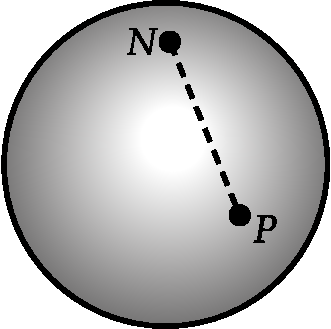
\includegraphics[height=3cm,width=3cm]{t335}
\end{figure}
\begin{tasks}(4)
	\task[\textbf{A.}] $R$
	\task[\textbf{B.}] $2 \sqrt{\frac{2}{5}} R$
	\task[\textbf{C.}]   $\sqrt{4 \pi} R$
	\task[\textbf{D.}] $\sqrt{2} R$
\end{tasks}
\begin{answer}$\left. \right. $\\
	\begin{figure}[H]
		\centering
		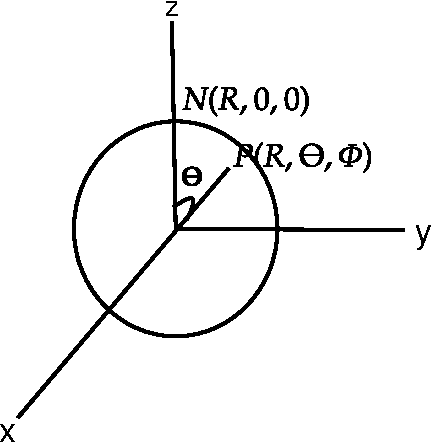
\includegraphics[height=3cm,width=5cm]{t1a}
	\end{figure}
$\begin{aligned} d &=\sqrt{(R \sin \theta \cos \phi)^{2}+(R \sin \theta \sin \phi)^{2}+(R \cos \theta-R)^{2}} \\ &=\sqrt{R^{2} \sin ^{2} \theta+R^{2}(1-\cos \theta)^{2}} \\ &=\sqrt{R^{2} \sin ^{2} \theta+R^{2}+R^{2} \cos ^{2} \theta-2 R^{2} \cos \theta} \\ &=\sqrt{2 R^{2}-2 R^{2} \cos \theta}=\sqrt{2 R^{2}(1-\cos \theta)} \\ &=\sqrt{4 R^{2} \sin ^{2} \theta / 2}=2 R \sin \theta / R \\ d_{\mathrm{rms}} &=\sqrt{\frac{\int d^{2} d S}{4 \pi R^{2}}} \end{aligned}$\\
$$
\begin{aligned}
\int d^{2} d S &=\int_{0}^{\pi} \int_{0}^{2 \pi} 2 R^{2}(1-\cos \theta) R^{2} \sin \theta d \phi d \theta \\
&=4 R^{4} \pi \int_{0}^{\pi}(1-\cos \theta) \sin \theta d \theta \\
&=4 \pi R^{4} \int_{0}^{\pi} \sin \theta d \theta=8 \pi R^{4} \\
d_{\mathrm{rms}} &=\sqrt{\frac{8 \pi R^{4}}{4 \pi R^{2}}}=\sqrt{2} R
\end{aligned}
$$\\
So,\\
	So the correct answer is \textbf{option(D)}
\end{answer}
\begin{minipage}{\textwidth}
	\question Consider a satellite orbiting the Earth in a circular orbit, as sketched in the figure on the right (not to scale). The satellite has four small thruster rockets, whose exhaust gases come out along\\
	(A) The forward direction,\\
	(B) The backward direction,\\
	(C) Radially inward towards the Earth's centre, and\\
	(D) Radially outward from the Earth's centre,\\
	If the satellite wants to increase its speed, while remaining in a circular orbit, and has fuel enough to keep only one thruster rocket in operation, it should fire the rocket marked
	(a) $\mathrm{A}$
	(b) $\mathrm{B}$
	(c) $\mathrm{C}$
	(d) $\mathrm{D}$
	\exyear{TIFR 2020}
\end{minipage}
\begin{figure}[H]
	\centering
	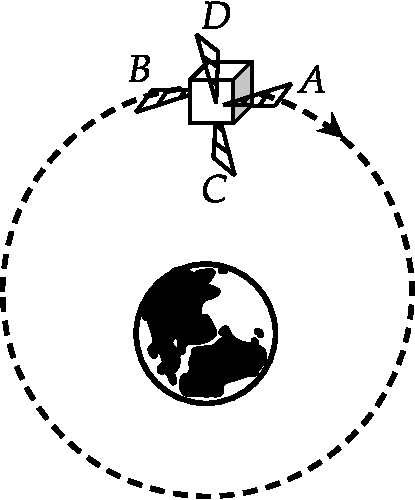
\includegraphics[height=5cm,width=4.3cm]{t336}
\end{figure}
\begin{tasks}(4)
	\task[\textbf{A.}] A
	\task[\textbf{B.}] B
	\task[\textbf{C.}] C
	\task[\textbf{D.}] D
\end{tasks}
\begin{answer}
	
	So the correct answer is \textbf{option(D)}
\end{answer}
\begin{minipage}{\textwidth}
	\question A particle of mass $m$ hangs from a light spring inside a lift (see figure). When the lift is at rest, the mass oscillates in the vertical direction with an angular frequency $2.5 \mathrm{rad} / \mathrm{s}$. Now consider the following situation.
	The suspended mass is at rest inside the lift which is descending vertically at a speed of $0.5 \mathrm{~m} / \mathrm{s}$. If the lift suddenly stops, the amplitude of oscillations of the mass will be
	\exyear{TIFR 2020}
\end{minipage}
\begin{figure}[H]
	\centering
	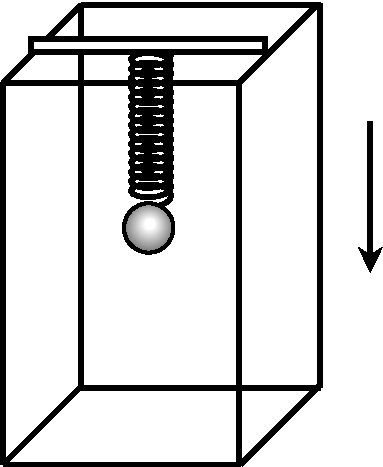
\includegraphics[height=4cm,width=3.1cm]{t337}
\end{figure}
\begin{tasks}(4)
	\task[\textbf{A.}] $0.20 \mathrm{~m}$
	\task[\textbf{B.}] $0.25 \mathrm{~m}$
	\task[\textbf{C.}] $0.05 \mathrm{~m}$
	\task[\textbf{D.}] $1.25 \mathrm{~m}$
\end{tasks}
\begin{answer}
	$$
	\omega=2.5 \mathrm{rad} / \mathrm{s}
	$$
	
	$\mathrm{kE}$ of bob $=\frac{1}{2} m(0.5)^{2}=\frac{m}{8}$
	
	when lift suddenly stops, this kE will become energy of oscillation
	
	$$
	\begin{aligned}
	\mathrm{kE} &=\frac{1}{2} m \omega^{2} A^{2} \\
	\frac{m}{8} &=\frac{1}{2} m(2.5)^{2} A^{2}
	\end{aligned}
	$$
	$$
	\begin{aligned}
	&=\frac{25}{8} m A^{2} \\
	&A=\sqrt{\frac{1}{25}}=\frac{1}{5}=0.2
	\end{aligned}
	$$
	
	So the correct answer is \textbf{option(A)}
\end{answer}
\begin{minipage}{\textwidth}
	\question Consider two planets $P_{1}$ and $P_{2}$ which can be modelled as uniform spheres of radii $R_{1}$ and $R_{2}$ respectively, and of the same material with the same density and other physical properties. If the maximum possible height of a conical mountain (of the same material) on these planets is denoted by $h_{1}$ and $h_{2}$ respectively $\left(h_{1} \square R_{1}, h_{2} \square R_{2}\right)$, then the ratio $\frac{h_{1}}{h_{2}}$ is
	\exyear{TIFR 2020}
\end{minipage}
\begin{tasks}(4)
	\task[\textbf{A.}] $\frac{R_{2}}{R_{1}}$
	\task[\textbf{B.}]   $\frac{R_{1}}{R_{2}}$
	\task[\textbf{C.}] $\frac{R_{2}^{2 / 3}}{R_{1}^{2 / 3}}$
	\task[\textbf{D.}]   $\frac{R_{1}^{2 / 3}}{R_{2}^{2 / 3}}$
\end{tasks}
\begin{answer}
	Using dimensional analysis $h \propto \frac{Y}{g \rho}$
	
	where $\quad Y=$ Young's modulus
	
	$g=$ acceleration due to gravity
	
	$\rho=$ density
	
	$Y$ and $\rho$ are properties of material, So, they are same for both planets
	
	$$
	g=\frac{G M}{R^{2}}=\frac{G \cdot \rho \cdot \frac{4}{3} \pi R^{3}}{R^{2}}=\frac{4 \pi \rho G R}{3}
	$$
	So,
	$$
	\frac{h_{1}}{h_{2}}=\frac{g_{1}}{g_{2}}=\frac{R_{1}}{R_{2}}
	$$
	So the correct answer is \textbf{option(A)}
\end{answer}
\begin{minipage}{\textwidth}
	\question A particle of rest mass $\sqrt{3} g$ emerges from a gun with a velocity $v=c / 4$. If the rest mass of the gun is $1 \mathrm{~kg}$, its approximate speed of recoil will be
	\exyear{TIFR 2020}
\end{minipage}
\begin{tasks}(4)
	\task[\textbf{A.}] $\frac{c}{1000}$
	\task[\textbf{B.}] $\frac{c}{2236}$
	\task[\textbf{C.}] $\frac{c}{1732}$
	\task[\textbf{D.}]   $\frac{c}{2309}$
\end{tasks}
\begin{answer}
	Linear momentum of particle
	$$
	\begin{aligned}
	p=m v &=\frac{m_{0}}{\sqrt{1-\frac{v^{2}}{c^{2}}}} v \\
	&=\frac{\sqrt{3}}{\sqrt{1-\frac{1}{16}}} \cdot \frac{c}{4} \times 10^{-3} \\
	&=\frac{c}{\sqrt{5}} \times 10^{-3}
	\end{aligned}
	$$
	Linear momentum of gun will be equal and opposite to that of particle
	
	$$
	\begin{array}{r}
	p=\frac{c}{\sqrt{5}} \times 10^{-3} \\
	\frac{1}{\sqrt{1-\frac{v^{2}}{c^{2}}}} \cdot v=\frac{c}{\sqrt{5}} \times 10^{-3}
	\end{array}
	$$
	$$
	\begin{aligned}
	&\Rightarrow \quad \frac{(v / c)^{2}}{\sqrt{1-\frac{v^{2}}{c^{2}}}}=\frac{10^{-6}}{5} \\
	&\left.\Rightarrow \quad v \approx \frac{10^{-3}}{\sqrt{5}} c=\frac{c}{2236}\right)^{2}=10^{-6}-10^{-6}\left(\frac{v}{c}\right)^{2} \\
	&\Rightarrow \quad v
	\end{aligned}
	$$
	So the correct answer is \textbf{option(B)}
\end{answer}
\begin{minipage}{\textwidth}
	\question Consider two concentric spheres of radii $a$ and $b$, where $a<b$ (see figure). The (shaded) space between thee two spheres is filled uniformly with total charge $Q$. The electric field at any point between thee two spheres at distance $r$ from the centre is given by
	\exyear{TIFR 2020}
\end{minipage}
\begin{figure}[H]
	\centering
	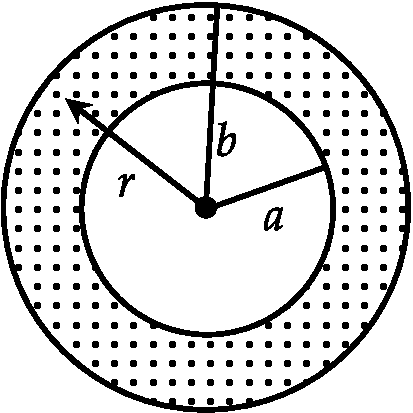
\includegraphics[height=4cm,width=4cm]{t338}
\end{figure}
\begin{tasks}(2)
	\task[\textbf{A.}] $\frac{Q}{4 \pi \in_{0}} \frac{r^{3}-a^{3}}{r^{2}\left(b^{3}-a^{3}\right)}$
	\task[\textbf{B.}] $\frac{Q}{4 \pi \in_{0}} \frac{1}{r^{2}}$
	\task[\textbf{C.}]   $\frac{Q}{4 \pi \epsilon_{0}}\left(\frac{b}{r^{4}}-\frac{a}{r^{4}}\right)^{2 / 3}$
	\task[\textbf{D.}]   zero
\end{tasks}
\begin{answer}
		So the correct answer is \textbf{option(A)}
\end{answer}
\begin{minipage}{\textwidth}
	\question A metallic wire of uniform cross- section and resistance $R$ is bent into a circle of radius $a$. The circular loop is placed in a magnetic field $\vec{B}(t)$ which is perpendicular to the plane of the wire. This magnetic field is uniform over space, but its magnitude decreases with time at a constant rate $k$, where
	$$
	k=-\frac{d|\vec{B}(t)|}{d t}
	$$
	The tension in the metallic wire is
	\exyear{TIFR 2020}
\end{minipage}
\begin{tasks}(4)
	\task[\textbf{A.}]   $\frac{\pi a^{3} k}{2 R}|\vec{B}(t)|$
	\task[\textbf{B.}]   $\frac{\pi a^{3} k}{R}|\vec{B}(t)|$
	\task[\textbf{C.}] 
	\task[\textbf{D.}]   Zero
\end{tasks}
\begin{answer}
	$$
	\text { Flux } \phi=B \pi a^{2}
	$$
	Emf induced, $\quad \varepsilon=\frac{-\partial \phi}{\partial t}=\pi a^{2} \frac{\partial B}{\partial t}$
	Current flowing in the loop
	$$
	i=\frac{\varepsilon}{R}=\frac{\pi a^{2} k}{R}
	$$
	Consider an element of the loop. \\
	$$
	d l=a d \theta
	$$
	Lorentz force acting on $d l$ length of loop
	\begin{figure}[H]
		\centering
		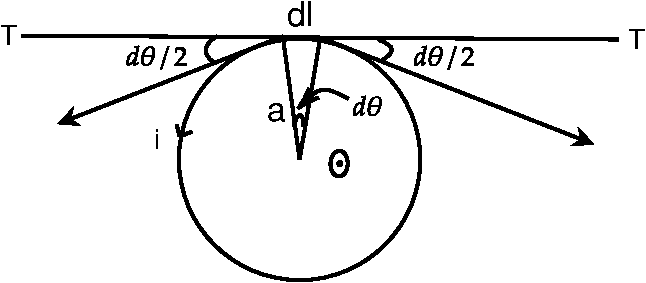
\includegraphics[height=3cm,width=5cm]{t 1g}
		
	\end{figure}
	$$
	d F=i d l B
	$$
	
	$$
	=\frac{\pi a^{2} k}{R} \cdot a d \theta B=\frac{\pi a^{3} k B d \theta}{R} \text { in radially outward direction }
	$$
	It will be balanced by tension in radially inward direction.
	$$	\begin{aligned}
	d F &=2 T \sin \frac{d \theta}{2}=T d \theta \\
	\frac{\pi a^{3} k B}{R} d \theta &=T d \theta \\
	T &=\frac{\pi a^{3} k B}{R}
	\end{aligned}
	$$
	So the correct answer is \textbf{option(B)}
\end{answer}
\begin{minipage}{\textwidth}
	\question Four students were asked to write down possible forms for the magnetic vector potential $\vec{A}(\vec{x})$ corresponding to a uniform magnetic field of magnitude $B$ along the positive $z$ direction. Three returned correct answers and one returned an incorrect answers. Their answers are reproduced below. Which was the incorrect answer?
	\exyear{TIFR 2020}
\end{minipage}
\begin{tasks}(2)
	\task[\textbf{A.}] $B x \hat{j}$
	\task[\textbf{B.}]   $-B y \hat{i}$
	\task[\textbf{C.}]   $\frac{1}{2}(B x \hat{i}-B y \hat{j})$
	\task[\textbf{D.}] $\frac{1}{2}(-B y \hat{i}+B x \hat{j})$
\end{tasks}
\begin{answer}
	(A)
$$
\begin{aligned}
\vec{B} &=\nabla \times \vec{A} \\
&=\left|\begin{array}{ccc}
\hat{i} & \hat{j} & \hat{k} \\
\frac{\partial}{\partial x} & \frac{\partial}{\partial y} & \frac{\partial}{\partial z} \\
A_{x} & A_{y} & A_{z}
\end{array}\right|=B \hat{k}
\end{aligned}
$$
$$
\begin{aligned}
\vec{A} &=B x \hat{j} \\
\vec{B} &=\left|\begin{array}{rrr}
\hat{i} & \hat{j} & \hat{k} \\
\frac{\partial}{\partial x} & \frac{\partial}{\partial y} & \frac{\partial}{\partial z} \\
0 & B x & 0
\end{array}\right|=B \hat{k}
\end{aligned}
$$
(B)
$$
\vec{A}=-B y \hat{i}
$$\\
$$
\begin{aligned}
\vec{B} &=\nabla \times \vec{A} \\
&=\left|\begin{array}{rrr}
\hat{i} & \hat{j} & \hat{k} \\
\frac{\partial}{\partial x} & \frac{\partial}{\partial y} & \frac{\partial}{\partial z} \\
-B y & 0 & 0
\end{array}\right| \\
&=B \hat{k}
\end{aligned}
$$
(C)
$$
\begin{aligned}
\vec{A} &=\frac{1}{2}(B x \hat{i}-B y \hat{j}) \\
\vec{B} &=\nabla \times \vec{A} \\
&=\left|\begin{array}{rrr}
\hat{i} & \hat{j} & \hat{k} \\
\frac{\partial}{\partial x} & \frac{\partial}{\partial y} & \frac{\partial}{\partial z} \\
\frac{1}{2} B x & -\frac{1}{2} B y & 0
\end{array}\right|=0
\end{aligned}
$$\\
(D)
$$
\begin{aligned}
\vec{A} &=\frac{1}{2}(-B x \hat{i}+B y \hat{j}) \\
\vec{B} &=\nabla \times \vec{A} \\
&=\left|\begin{array}{rrr}
\frac{\partial}{\partial x} & \frac{\partial}{\partial y} & \frac{\partial}{\partial z} \\
-\frac{1}{2} B y & \frac{1}{2} B x & 0
\end{array}\right|=B \hat{k}
\end{aligned}
$$
	So the correct answer is \textbf{option(C)}
\end{answer}
\begin{minipage}{\textwidth}
	\question The components of the electric and magnetic fields corresponding to a plane electromagnetic field propagating in vacuum satisfy\\
	$E_{x}=E_{y}=-E_{z}=\frac{|\vec{E}|}{\sqrt{3}}$
	$B_{x}=-B_{y}=\frac{|\vec{B}|}{\sqrt{2}}$
	$B_{z}=0$\\
	A unit vector along the direction of propagation of the plane wave is
	\exyear{TIFR 2020}
\end{minipage}
\begin{tasks}(4)
	\task[\textbf{A.}] $\frac{\hat{i}+\hat{j}+2 \hat{k}}{\sqrt{6}}$
	\task[\textbf{B.}] $-\frac{\hat{i}+\hat{j}+2 \hat{k}}{\sqrt{6}}$
	\task[\textbf{C.}] $\frac{2 \hat{i}-2 \hat{j}+\hat{k}}{\sqrt{3}}$
	\task[\textbf{D.}] $-\frac{2 \hat{i}-2 \hat{j}+\hat{k}}{\sqrt{3}}$
\end{tasks}
\begin{answer}
	$$
	\begin{aligned}
	&\vec{E}=|\vec{E}|\left(\frac{1}{\sqrt{3}} \hat{i}+\frac{1}{\sqrt{3}} \hat{j}-\frac{1}{\sqrt{3}} \hat{k}\right) \\
	&\vec{B}=|\vec{B}|\left(\frac{1}{\sqrt{2}} \hat{i}-\frac{1}{\sqrt{2}} \hat{j}\right)
	\end{aligned}
	$$
	Unit vector in the direction of propagation of em wave 
	$$
	\hat{n} \| \vec{E} \times \vec{B}
	$$
	So,
	$$
	\begin{aligned}
	\hat{n} &=\left|\begin{array}{ccc}
	\hat{i} & \hat{j} & \hat{k} \\
	\frac{1}{\sqrt{3}} & \frac{1}{\sqrt{3}} & -\frac{1}{\sqrt{3}} \\
	\frac{1}{\sqrt{2}} & -\frac{1}{\sqrt{2}} & 0
	\end{array}\right| \\
	&=-\frac{1}{\sqrt{6}} \hat{i}-\frac{1}{\sqrt{6}} \hat{j}-\frac{2}{\sqrt{6}} \hat{k} \\
	&=-\left(\frac{\hat{i}+\hat{j}+2 \hat{k}}{\sqrt{6}}\right)
	\end{aligned}
	$$
	So the correct answer is \textbf{option(B)}
\end{answer}
\begin{minipage}{\textwidth}
	\question A gas has the following equation of state
	$$
	U=\frac{a S^{5}}{N^{2} V^{2}}
	$$
	where $U$ is the internal energy, $V$ is the volume and $N$ is the number of particles. Here $a$ is a constant of the appropriate dimension. It follows that the equation of state of this gas relating its pressure $P$ to its temperature $T$ and its density $\rho=\frac{N}{V}$ is given by
	\exyear{TIFR 2020}
\end{minipage}
\begin{tasks}(2)
	\task[\textbf{A.}] $\frac{P^{5}}{T^{5} \rho^{2}}=$ constant
	\task[\textbf{B.}] $\frac{P^{5}}{T^{4} \rho^{3}}=$ constant
	\task[\textbf{C.}] $\frac{P}{T \rho}=$ constant
	\task[\textbf{D.}] $\frac{P^{3}}{T^{2} \rho^{3}}=$ constant
\end{tasks}
\begin{answer}
	So the correct answer is \textbf{option(A)}
\end{answer}
\begin{minipage}{\textwidth}
	\question An ideal gas is passed through a cyclic process where the corresponding changes in the thermodynamic potentials are plotted on the adjoining graph. Here $U$ is the internal energy and $F$ is the Helmholtz free energy.
	The efficiency of this cycle is given by
	\exyear{TIFR 2020}
\end{minipage}
\begin{figure}[H]
	\centering
	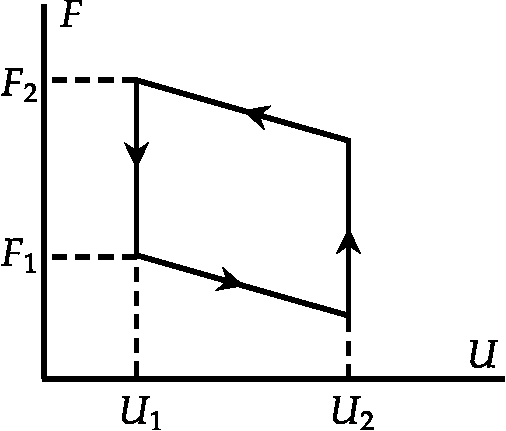
\includegraphics[height=4cm,width=4.5cm]{t339}
\end{figure}
\begin{tasks}(2)
	\task[\textbf{A.}] $1-\frac{U_{1}}{U_{2}}$
	\task[\textbf{B.}] $1-\exp \left(-\frac{F_{2}}{F_{1}}\right)$
	\task[\textbf{C.}]   $1-\frac{U_{1}}{U_{2}} \exp \left(-\frac{F_{2}}{F_{1}}\right)$
	\task[\textbf{D.}]   $\exp \left(\frac{U_{1}}{U_{2}}\right)-\exp \left(-\frac{F_{2}}{F_{1}}\right)$
\end{tasks}
\begin{answer}
	For ideal gas, $U \propto T$
	$$
	\eta=1-\frac{T_{2}}{T_{1}}=1-\frac{U_{1}}{U_{2}}
	$$
	
	So the correct answer is \textbf{option(A)}
\end{answer}
\begin{minipage}{\textwidth}
	\question The mean free path $\lambda$ of molecules of a gas at room temperature is given approximately by
	$$
	\lambda=\frac{1}{n \sigma}
	$$
	where $n$ is the number density of the molecules and $\sigma$ is the collision cross-section of two molecules. It follows that the mean free path of air molecules at normal temperature and pressure is of order
	\exyear{TIFR 2020}
\end{minipage}
\begin{tasks}(4)
	\task[\textbf{A.}] $500 \mu \mathrm{m}$
	\task[\textbf{B.}] $50 \mathrm{~nm}$
	\task[\textbf{C.}] $0.5 \mathrm{~nm}$
	\task[\textbf{D.}] $500 \mathrm{fm}$
\end{tasks}
\begin{answer}
	
	So the correct answer is \textbf{option(B)}
\end{answer}
\begin{minipage}{\textwidth}
	\question Four students are asked to draw on the same semi-logarithmic plot the energy distributions $f(E)$ of a classical gas (with a solid line), a boson gas (with a dashed line) and a fermion gas (with a dash-dot line) respectively, each as a function of energy $E .$ Only one student's answer was correct. The graphs submitted by the four students are given below. The correct one is
	\exyear{TIFR 2020}
\end{minipage}
\begin{tasks}(2)
	\task[\textbf{A.}] \begin{figure}[H]
		\centering
		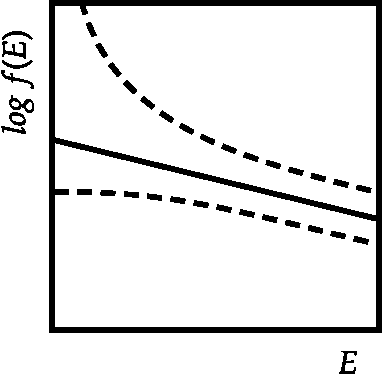
\includegraphics[height=4cm,width=4cm]{t340}
	\end{figure}
	\task[\textbf{B.}] \begin{figure}[H]
		\centering
		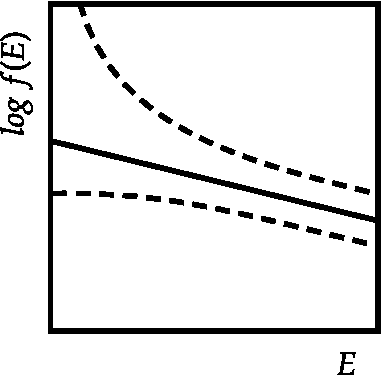
\includegraphics[height=4cm,width=4cm]{t341}
	\end{figure}
	\task[\textbf{C.}] \begin{figure}[H]
		\centering
		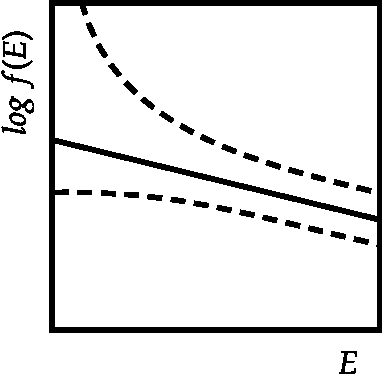
\includegraphics[height=4cm,width=4cm]{t342}
	\end{figure}
	\task[\textbf{D.}] \begin{figure}[H]
		\centering
		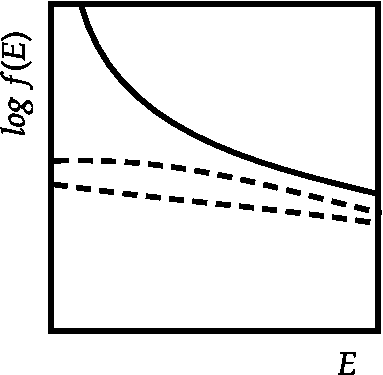
\includegraphics[height=4cm,width=4cm]{t343}
	\end{figure}
\end{tasks}
\begin{answer}
	So the correct answer is \textbf{option(A)}
\end{answer}
\begin{minipage}{\textwidth}
	\question The wave function of a particle subjected to a three-dimensional spherically-symmetric potential $V(r)$ is given by
	$$
	\psi(\vec{x})=(x+y+3 z) f(r)
	$$
	the expectation value for the operator $\vec{L}^{2}$ for this state is
	\exyear{TIFR 2020}
\end{minipage}
\begin{tasks}(4)
	\task[\textbf{A.}]   $\hbar^{2}$
	\task[\textbf{B.}] $2 \hbar^{2}$
	\task[\textbf{C.}] $5 \hbar^{2}$
	\task[\textbf{D.}] $11 \hbar^{2}$
\end{tasks}
\begin{answer}
	So the correct answer is \textbf{option(B)}
\end{answer}
\begin{minipage}{\textwidth}
	\question A fermion of mass $m$, moving in two dimensions, is strictly confined inside a square box of side $\ell$. The potential inside is zero. A measurement of the energy of the fermion yields the result
	$$
	E=\frac{65 \pi^{2} \hbar^{2}}{2 m \ell^{2}}
	$$
	The degeneracy of this energy state is
	\exyear{TIFR 2020}
\end{minipage}
\begin{tasks}(4)
	\task[\textbf{A.}] 2
	\task[\textbf{B.}] 4
	\task[\textbf{C.}] 8
	\task[\textbf{D.}] 16
\end{tasks}
\begin{answer}
	$$
	E=\frac{\hbar^{2} \pi^{2}}{2 m a^{2}}\left(n_{x}^{2}+n_{y}^{2}\right)=\frac{65 \hbar^{2} \pi^{2}}{2 m a^{2}}
	$$
	So,
	$$
	n_{x}^{2}+n_{y}^{2}=65
	$$
	So, $\left(n_{x}, n_{y}\right)$ can be $(8,1),(1,8),(7,4),(4,7)$.
	
	If we consider spin then there will be 8 degeneracy states.
	
	So the correct answer is \textbf{option(C)}
\end{answer}
\begin{minipage}{\textwidth}
	\question A sample of hydrogen gas was placed in a discharge tube and its spectrum was measured using a high-resolution spectrometer. The $H_{\alpha}$ line in the spectrum was found to be split into two lines, a high intensity line at $656.28 \mathrm{~nm}$, and a low intensity line at $656.01 \mathrm{~nm}$. This indicates that the hydrogen sample was contaminated with
	\exyear{TIFR 2020}
\end{minipage}
\begin{tasks}(2)
	\task[\textbf{A.}] Deuterium
	\task[\textbf{B.}] Tritium
	\task[\textbf{C.}] Helium
	\task[\textbf{D.}] Water vapour
\end{tasks}
\begin{answer}
		$$
	E_{n}=-\frac{\mu e^{4}}{8 n^{2} h^{2} \epsilon_{0}^{2}}
	$$
	
	For $H_{\alpha}$ line
	
	$$
	\frac{\lambda c}{\lambda}=E_{3}-E_{2}=\frac{\mu e^{4}}{8 h^{2} \in_{0}^{2}}\left(\frac{1}{4}-\frac{1}{9}\right)
	$$
	
	So,
	
	$$
	\frac{\lambda}{\lambda^{\prime}}=\frac{\mu^{\prime}}{\mu}
	$$
	
	$\Rightarrow \quad \frac{656.28}{656.01}=\frac{\mu^{\prime}}{\mu}=\frac{\frac{x m_{p} \cdot m_{e}}{x m_{p}+m_{e}}}{\frac{m_{p} \cdot m_{e}}{m_{p}+m_{e}}}=\frac{x\left(m_{p}+m_{e}\right)}{x m_{p}+m_{e}}$
	
	$$
	=\frac{x\left(\frac{m_{p}}{m_{e}}+1\right)}{x \frac{m_{p}}{m_{e}}+1}=\frac{1841 x}{1840 x+1}
	$$
	
	$\Rightarrow \quad 656.28 \times 1840 x+656.28=656.01 \times 1841 x$
	
	$\Rightarrow \quad 1207552.2 x+656.28=1207714.41 x$
	
	$\Rightarrow \quad x=\frac{656.28}{162.21}=4.046$
	
	So, nucleus of unknown species will contain 4 nucleons. It must be He\\
	So the correct answer is \textbf{option(C)}
\end{answer}
\begin{minipage}{\textwidth}
	\question The momentum operator
	$$
	i \hbar \frac{d}{d x}
	$$
	acts on a wavefunction $\psi(x)$. This operator is Hermitian
	\exyear{TIFR 2020}
\end{minipage}
\begin{tasks}(1)
	\task[\textbf{A.}]   Provided the wavefunction $\psi(x)$ is normalized
	\task[\textbf{B.}]   Provided the wavefunction $\psi(x)$ and derivate $\psi^{\prime}(x)$ are continuous everywhere
	\task[\textbf{C.}] Provided the wavefunction $\psi(x)$ vanishes as $x \rightarrow \pm \infty$
	\task[\textbf{D.}] By its very definition
\end{tasks}
\begin{answer}
	So the correct answer is \textbf{option(C)}
\end{answer}

\begin{minipage}{\textwidth}
	\question \begin{figure}[H]
		\centering
		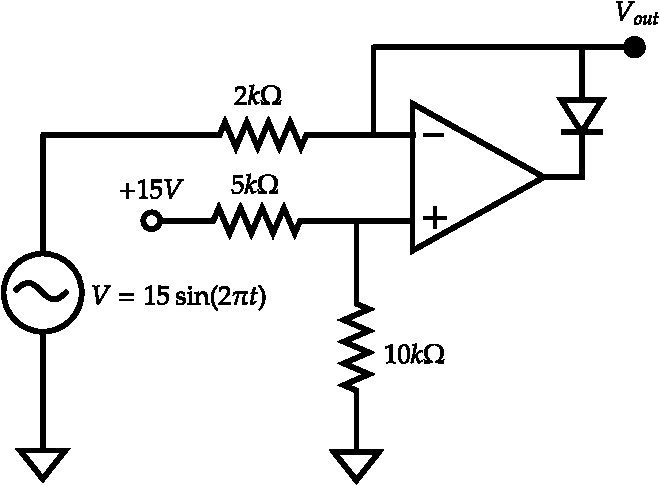
\includegraphics[height=5cm,width=6cm]{t345}
	\end{figure}
	In the above circuit, which of the following is the maximum value, in Volts, of voltage at $V_{\text {out }} ?$
	\exyear{TIFR 2020}
\end{minipage}
\begin{tasks}(4)
	\task[\textbf{A.}] 18
	\task[\textbf{B.}] 15
	\task[\textbf{C.}] 0
	\task[\textbf{D.}] 5
\end{tasks}
\begin{answer}
	So the correct answer is \textbf{option(A)}
\end{answer}
\begin{minipage}{\textwidth}
	\question A badly-designed voltmeter is modelled as an ideal voltmeter with a large resistor $(R)$ and a large capacitor $(C)$ connected in parallel to it. Given this information, which of the following statements describes what happens when this voltmeter is connected to a DC voltage source with voltage $V$ and internal resistance $r(r \square R)$ ?
	\exyear{TIFR 2020}
\end{minipage}
\begin{tasks}(1)
	\task[\textbf{A.}] The reading on the voltameter rises slowly and becomes steady at a value slightly less than $V$
	\task[\textbf{B.}] The reading on the voltameter starts at a value slightly less than $V$ and slowly falls to zero.
	\task[\textbf{C.}] The reading on the voltameter rises slowly to maximum value close to $V$ and then slowly goes to zero.
	\task[\textbf{D.}]   The reading on the voltameter reads zero even when connected to the voltage source.
\end{tasks}
\begin{answer}
	So the correct answer is \textbf{option(A)}
\end{answer}
\begin{minipage}{\textwidth}
	\question An OR gate, a NOR gate and an XOR gate are to be constructed using only NAND gates. If the minimum number of NAND gates needed to construct OR, NOR nd XOR gates is denoted $n(\mathrm{OR}), n(\mathrm{NOR})$ and $n(\mathrm{XOR})$ respectively, then
	\exyear{TIFR 2020}
\end{minipage}
\begin{tasks}(2)
	\task[\textbf{A.}] $n(\mathrm{NOR})=n(\mathrm{XOR})>n(\mathrm{OR})$
	\task[\textbf{B.}]   $n(\mathrm{NOR})=n(\mathrm{XOR})=n(\mathrm{OR})$
	\task[\textbf{C.}] $n(\mathrm{NOR})>n(\mathrm{XOR})>n(\mathrm{OR})$
	\task[\textbf{D.}]   $n(\mathrm{NOR})<n(\mathrm{XOR})=n(\mathrm{OR})$
\end{tasks}
\begin{answer}
	OR Gate\\$y=A+B=\overline{\bar{A} \bar{B}}$
	\begin{figure}[H]
		\centering
		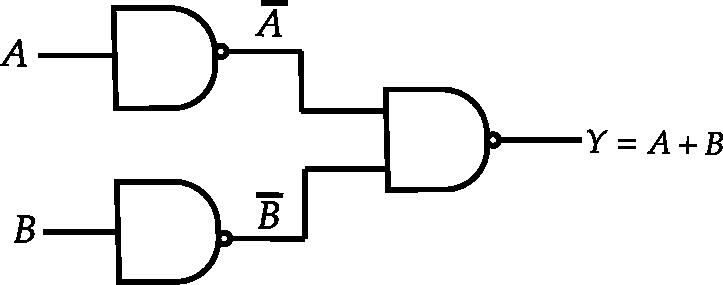
\includegraphics[height=3cm,width=5cm]{t 1b}\\
	\end{figure}
So, $n(\mathrm{OR})=3$\\
NOR Gate\\
\begin{figure}[H]
	\centering
	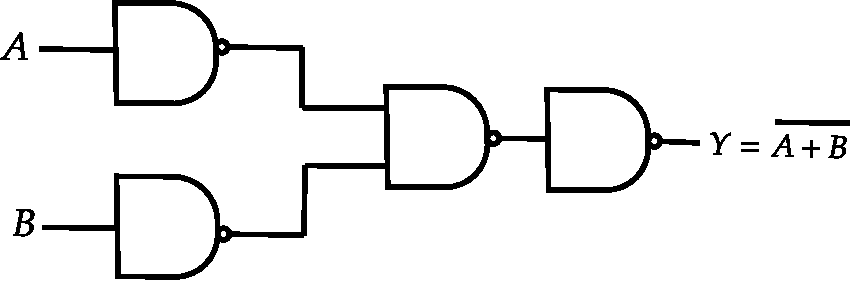
\includegraphics[height=4cm,width=5cm]{t 1c}\\
\end{figure}
	So, $n(\mathrm{NOR})=4$\\
XOR Gate\\
\begin{figure}[H]
	\centering
	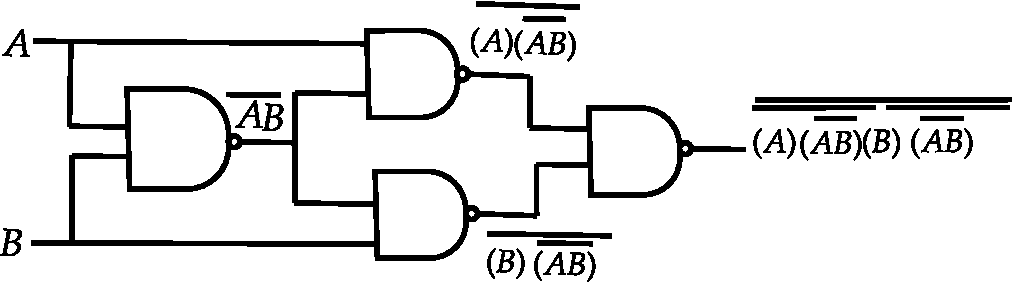
\includegraphics[height=3cm,width=5cm]{t 1d}
	\end{figure}
$\begin{aligned} y &=\overline{\overline{(A)(\overline{A B})} \overline{(B)(\overline{A B})}} \\ &=(A)(\overline{A B})+(B)(\overline{A B}) \\ &=A(\bar{A}+\bar{B})+B(\bar{A}+\bar{B}) \\ &=A \bar{B}+B \bar{A} \\ &=\bar{A} B+A \bar{B} \end{aligned}$\\
So, $n(\mathrm{XOR})=4$\\ Hence,$n(\mathrm{XOR})=n(\mathrm{NOR})>n(\mathrm{OR})$\\
	So the correct answer is \textbf{option(A)}
\end{answer}
\begin{minipage}{\textwidth}
	\question On passing electric current, a tungsten filament is emitting electrons by thermionic emission. In order to maintain the energy of the electron beam obtained from this source at a value approximately $100 \mathrm{eV}$, which of the following methods will work in practice?
	\exyear{TIFR 2020}
\end{minipage}
\begin{tasks}(1)
	\task[\textbf{A.}]   Float the filament at $-100$ Volts with a grounded aperture in front of it.
	\task[\textbf{B.}] Heat the filament so that the emitted electrons will have $100 \mathrm{eV}$ kinetic energy due to temperature.
	\task[\textbf{C.}] Apply a $+100$ Volts potential with respect to the filament potential to an aperture kept very close to the filament.
	\task[\textbf{D.}] Use an appropriate magnetic field to draw out the electron beam at the desired energy without applying any electric field.
\end{tasks}
\begin{answer}
	So the correct answer is \textbf{option(A)}
\end{answer}
\begin{minipage}{\textwidth}
	\question A two-dimensional electrostatic field is defined as
	$$
	\vec{E}(x, y)=-x \hat{i}+y \hat{j}
	$$
	A correct diagram for the lines of force is
	\exyear{TIFR 2020}
\end{minipage}
\begin{tasks}(2)
	\task[\textbf{A.}] \begin{figure}[H]
		\centering
		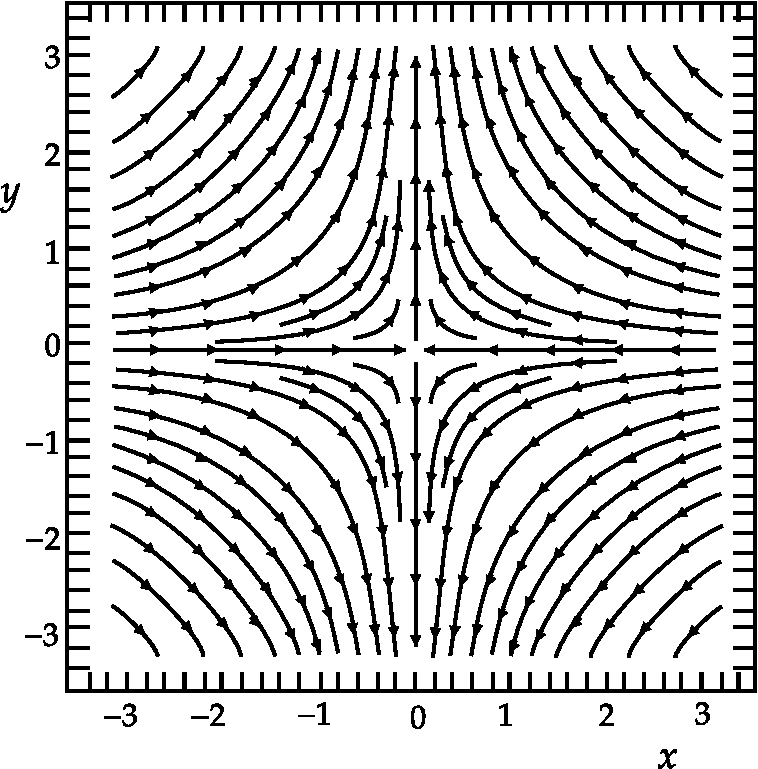
\includegraphics[height=6cm,width=6cm]{t346}
	\end{figure}
	\task[\textbf{B.}] \begin{figure}[H]
		\centering
		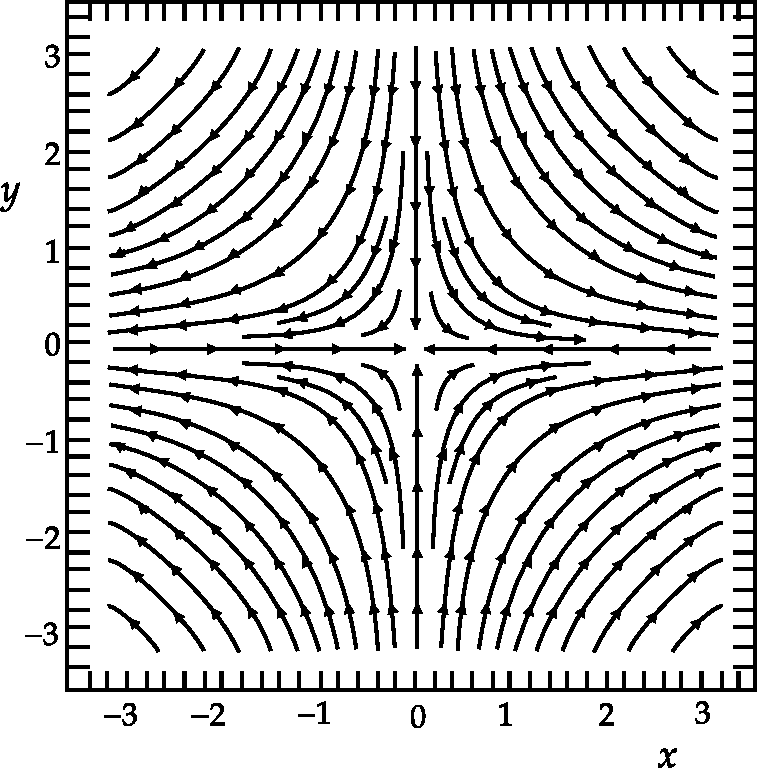
\includegraphics[height=6cm,width=6cm]{t347}
	\end{figure}
	\task[\textbf{C.}] \begin{figure}[H]
		\centering
		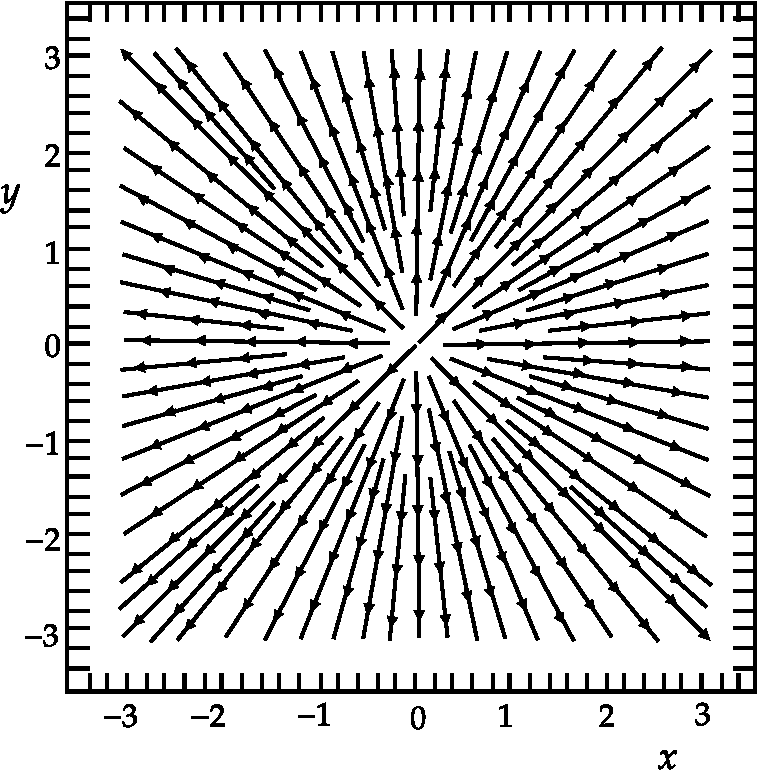
\includegraphics[height=6cm,width=6cm]{t348}
	\end{figure}
	\task[\textbf{D.}] \begin{figure}[H]
		\centering
		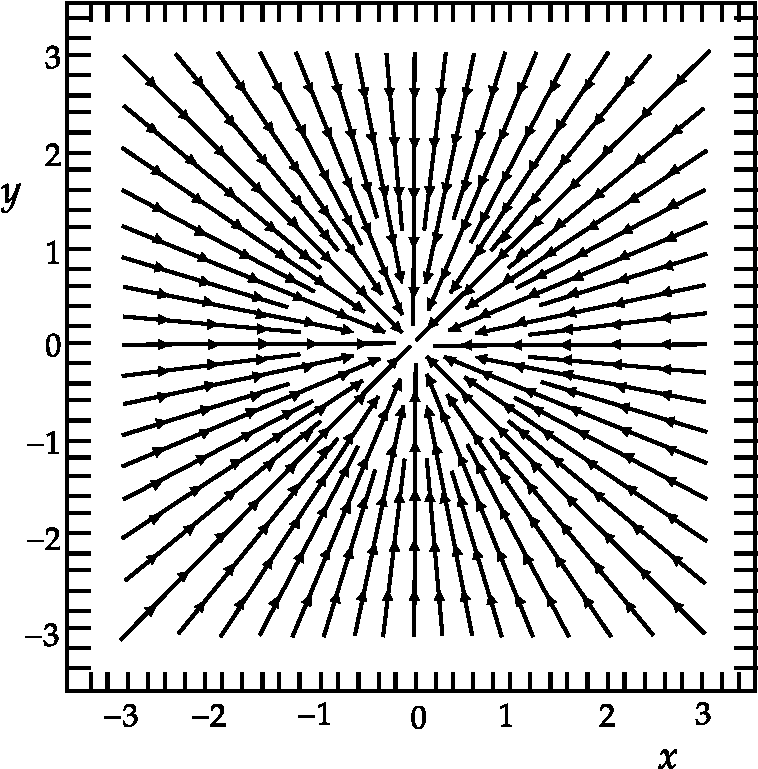
\includegraphics[height=6cm,width=6cm]{t349}
	\end{figure}
\end{tasks}
\begin{answer}
	$$
	\nabla \cdot \vec{E}=0
	$$
	So, $\vec{E}$ is divergenceless\\
	(iii) \& (iv) is incorrect.\\
	For negative side of $x$-axis, $E$ is positive and the test charge will move towards right. \\So, (a) is correct.\\
	So the correct answer is \textbf{option(A)}
\end{answer}
\begin{minipage}{\textwidth}
	\question The sum of the infinite series $S=1+\frac{3}{5}+\frac{6}{25}+\frac{10}{125}+\frac{15}{625}+\ldots .$ is given by
	\exyear{TIFR 2020}
\end{minipage}
\begin{tasks}(4)
	\task[\textbf{A.}] $S=\frac{125}{64}$
	\task[\textbf{B.}] $S=\frac{25}{16}$
	\task[\textbf{C.}] $S=\frac{25}{24}$
	\task[\textbf{D.}]   $S=\frac{16}{25}$
\end{tasks}
\begin{answer}
	$$
	S=\frac{1}{5}+\frac{3}{25}+\frac{6}{125}+\frac{10}{625}+\ldots
	$$
	
	$\frac{S}{5}=\frac{1}{5}+\frac{2}{25}+\frac{6}{125}+\frac{10}{625}+\ldots$
	
	$S^{\prime}=\frac{4}{5} S=1+\frac{1}{5}+\frac{3}{25}+\frac{6}{125}+\frac{10}{625}+\ldots$
	
	$\frac{S^{\prime}}{5}=\frac{1}{5}+\frac{2}{25}+\frac{6}{125}+\frac{10}{625}+\ldots$
	
	$\frac{4}{5} S^{\prime}=1+\frac{1}{5}+\frac{2}{25}+\frac{6}{125}+\frac{10}{625}+\ldots .$
	
	$$
	\begin{aligned}
	&=\frac{1}{1-\frac{1}{5}}=\frac{5}{4} \\
	S^{\prime} &=\frac{4}{5} S=\frac{25}{16} \\
	S &=\frac{125}{64}
	\end{aligned}
	$$
	So the correct answer is \textbf{option(A)}
\end{answer}
\begin{minipage}{\textwidth}
	\question A roundabout rotating base is a heavy uniform disc of radius $2 \mathrm{~m}$ and mass $400 \mathrm{~kg}$ has a central pillar and handles which are of negligible mass (see figure). The roundabout is set rotating at a steady rate of 20 r.p.m.\\
	Four small children, of mass $10 \mathrm{~kg}, 20 \mathrm{~kg}, 30 \mathrm{~kg}$ and $40 \mathrm{~kg}$ respectively, step gently on to the edge of thee roundabout, each with velocity $7.2 \mathrm{~km} / \mathrm{hr}$ along a tangential direction and cling to the handles. After holding on for some time, the children step gently off the roundabout with the same velocity, but this time in a radial direction.\\
	Neglecting all effects of friction and air drag the final rate of rotation of the roundabout will be about
	\exyear{TIFR 2020}
\end{minipage}
\begin{figure}[H]
	\centering
	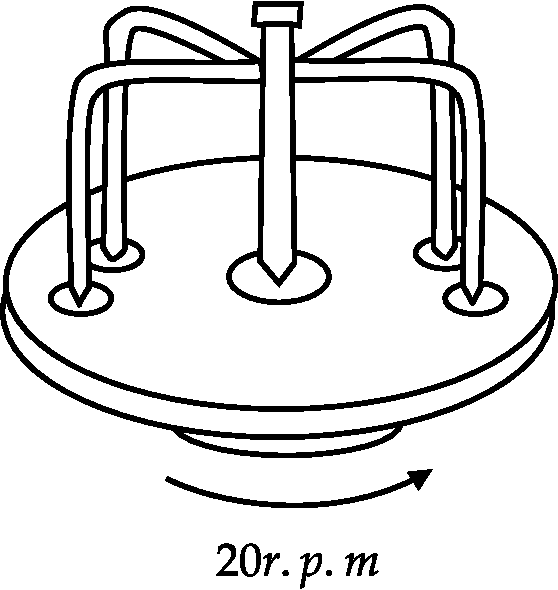
\includegraphics[height=4.7cm,width=5cm]{t350}
\end{figure}
\begin{tasks}(4)
	\task[\textbf{A.}] 28 r.p.m
	\task[\textbf{B.}] 25 r.p.m
	\task[\textbf{C.}] 36 r.p.m
	\task[\textbf{D.}] 21 r.p.m
\end{tasks}
\begin{answer}$\left. \right. $\\
	$\begin{aligned} V &=7.2 \mathrm{~km} / \mathrm{hr} \\ &=\frac{7.2 \times 1000}{3600}=2 \mathrm{~m} / \mathrm{s} \\ \omega &=2 \mathrm{rpm}=\frac{20 \times 2 \pi}{60}=\frac{2}{3} \pi \mathrm{rad} / \mathrm{s} \end{aligned}$\\
	Conserving angular momentum\\
	$\begin{aligned} \frac{1}{2} \times 400 \times 4 \times\left(\frac{2 \pi}{3}\right)+10 \times 2 \times 2+20 \times 2 \times 2+30 \times 2 \times 2+40 \times 2 \times 2 \\ &=\frac{1}{2} \times 400 \times 4 \omega \\ \Rightarrow \quad \frac{1600}{3} \pi+400 &=800 \omega \\ \omega &=\frac{2}{3} \pi+0.5 \\ \omega &=\left(\frac{2}{3} \pi+0.5\right) \times \frac{60}{2 \pi} \\ &=20+\frac{15}{\pi}=24.777 \mathrm{rpm} \end{aligned}$\\
	So the correct answer is \textbf{option(B)}
\end{answer}
\begin{minipage}{\textwidth}
	\question In the laboratory frame, a particle at rest starts moving with a speed $\frac{c}{2}$ from one corner of a square (see figure) and traverses the four sides of the square so that it returns to its original position. At each corner, it changes direction without any change in speed.\\
	If the entire square now moves with a speed $\frac{c}{3}$ in the laboratory frame, as indicated in the figure, the speed of the particle (in the laboratory frame) when it returns to its original position will be
	\exyear{TIFR 2020}
\end{minipage}
\begin{figure}[H]
	\centering
	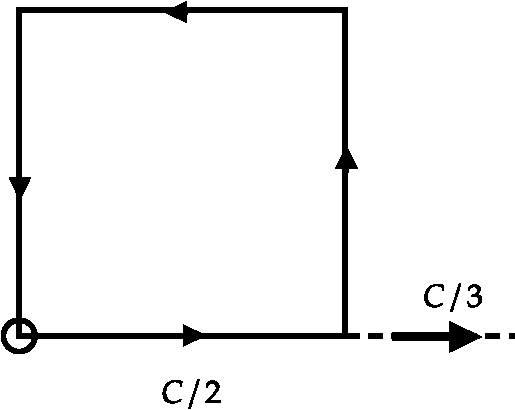
\includegraphics[height=3cm,width=4cm]{t351}
\end{figure}
\begin{tasks}(4)
	\task[\textbf{A.}] $\frac{2 \sqrt{2} c}{15}$
	\task[\textbf{B.}] $\frac{c}{5}$
	\task[\textbf{C.}]   $\frac{2 \sqrt{2} c}{3}$
	\task[\textbf{D.}] $\frac{c}{5 \sqrt{3}}$
\end{tasks}
\begin{answer}$\left. \right. $\\
	$\begin{aligned} v_{x}^{\prime} &=\frac{v_{x}-v}{1-\frac{v v_{x}}{v^{2}}} \\ &=\frac{\frac{c}{2}-\frac{c}{3}}{1-\left(\frac{c}{2} \cdot \frac{c}{3}\right) \frac{1}{c^{2}}}=\frac{c}{5} \end{aligned}$\\
	So the correct answer is \textbf{option(B)}
\end{answer}
\begin{minipage}{\textwidth}
	\question A light rigid insulating rod of length $\ell$ is suspended horizontally from a rigid frictionless pivot at one of the ends (see figure). At a vertical distance $h$ below the rod there is an infinite plane conducting plane, which is grounded.\\
	\begin{figure}[H]
		\centering
		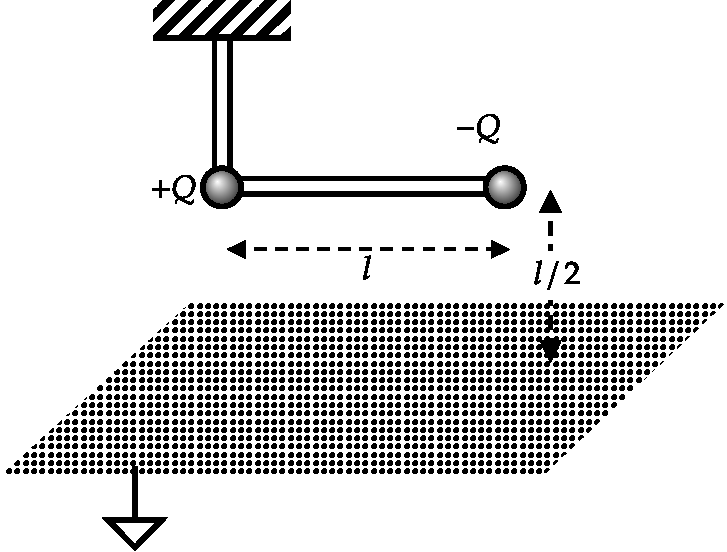
\includegraphics[height=4.5cm,width=6cm]{t352}
	\end{figure}
	If two small, light spherical conductors are attached at the ends of the rod and given charges $+Q$ and $-Q$ as indicated in the figure, the torque on the rod will be
	\exyear{TIFR 2020}
\end{minipage}
\begin{tasks}(4)
	\task[\textbf{A.}] $\frac{Q^{2}}{4 \pi \in_{0} \ell} \hat{k}$
	\task[\textbf{B.}] $-\frac{Q^{2}}{4 \pi \in_{0} \ell} \hat{k}$
	\task[\textbf{C.}] $\frac{(4-\sqrt{2})}{16 \pi \in_{0}} \frac{Q^{2}}{\ell} \hat{k}$
	\task[\textbf{D.}] $-\frac{(4-\sqrt{2})}{16 \pi \in_{0}} \frac{Q^{2}}{\ell} \hat{k}$
\end{tasks}
\begin{answer}$\left. \right. $\\
	\begin{figure}[H]
		\centering
		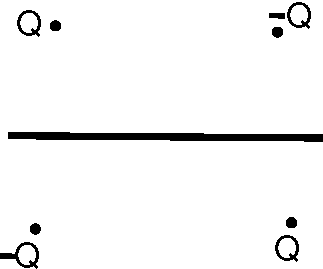
\includegraphics[height=3cm,width=4cm]{t 1p}
	\end{figure}
	Torque on rod
	$$
	\begin{aligned}
	\tau &=\frac{Q^{2}}{4 \pi \epsilon_{0} l^{2}} \cdot l-\frac{Q^{2}}{4 \pi \epsilon_{0}(\sqrt{2} l)^{2}} \cdot \frac{l}{\sqrt{2}} \\
	&=\frac{Q^{2}}{4 \pi \epsilon_{0} l}\left(1-\frac{1}{2 \sqrt{2}}\right) \\
	&=\frac{Q^{2}}{16 \pi \epsilon_{0} l}(4-\sqrt{2}) \text { Clockwise } \\
	\bar{\tau} &=\frac{Q^{2}}{16 \pi \epsilon_{0} l}(4-\sqrt{2})(-\hat{k})
	\end{aligned}
	$$
	In vector form,\\
	So the correct answer is \textbf{option(D)}
\end{answer}
\begin{minipage}{\textwidth}
	\question The magnitude vector potential $\vec{A}=A_{x} \hat{i}+A_{y} \hat{j}+A_{z} \hat{k}$ is defined in a region $R$ of space by $A_{x}=5 \cos \pi y$
	$$
	A_{y}=2+\sin \pi x
	$$
	$$
	A_{z}=0
	$$
	in an appropriate unit.
	If $L$ be a square loop of wire in the $x-y$ plane, with its end at
	$(0, \quad 0)$
	$(0,0.25)$
	$(0.25, \quad 0.25)$
	$(0.25, \quad 0)$
	In appropriate unit and it lies entirely in the region $R$, the numerical value of the flux of the above magnetic field (in the same units) passing through $L$ is
	\exyear{TIFR 2020}
\end{minipage}
\begin{tasks}(4)
	\task[\textbf{A.}] $0.543$
	\task[\textbf{B.}] $3.31$
	\task[\textbf{C.}] $-0.75$
	\task[\textbf{D.}] zero
\end{tasks}
\begin{answer}
	$$
	\begin{aligned}
	\vec{B} &=\nabla \times \vec{A} \\
	&=\left|\begin{array}{ccc}
	\hat{i} & \hat{j} & \hat{k} \\
	\frac{\partial}{\partial x} & \frac{\partial}{\partial y} & \frac{\partial}{\partial z} \\
	5 \cos \pi y & 2+\sin \pi x & 0
	\end{array}\right| \\
	&=(\pi \cos \pi x+5 \pi \sin \pi y) \hat{k}
	\end{aligned}
	$$
	
	Flux, $\phi=\int \vec{B} \cdot \hat{n} d S$
	
	$$
	\begin{aligned}
	&=\int_{0}^{1 / 41 / 4} \int_{0}^{1 / 4}(\pi \cos \pi x+5 \pi \sin \pi y) d x d y \\
	&=\int_{0}^{1 / \sin \pi x+\left.5 \pi x \sin \pi y\right|_{0} ^{1 / 4} d y} \\
	&=\int_{0}^{1 / 4}\left(\frac{1}{\sqrt{2}}+\frac{5 \pi}{4} \sin \pi y\right) d y \\
	&=\frac{y}{\sqrt{2}}-\left.\frac{5}{4} \cos \pi y\right|_{0} ^{1 / 4} \\
	&=\frac{1}{4 \sqrt{2}}-\frac{5}{4 \sqrt{2}}+\frac{5}{4} \\
	&=\frac{5}{4}-\frac{1}{\sqrt{2}}=0.543
	\end{aligned}
	$$
	So the correct answer is \textbf{option(A)}
\end{answer}
\begin{minipage}{\textwidth}
	\question The volume $V$ of a rectangular box is divided into two equal parts by a solid non permeable partition $P$. On one side of the partition $P$ there is a vacuum, while the other side is filled with a real gas having equation of state
	$$
	p V e^{a / R T V}=n R T
	$$
	where $a$ and $b$ are constants, The gas was initially at a uniform temperature $T_{0}$. Then the partition $P$ was removed instantaneously, and the gas was allowed to expand to fill the full volume of the box and come to equilibrium. The final temperature of the gas, in term of its specific heat $C_{v}$ will be
	\exyear{TIFR 2020}
\end{minipage}
\begin{figure}[H]
	\centering
	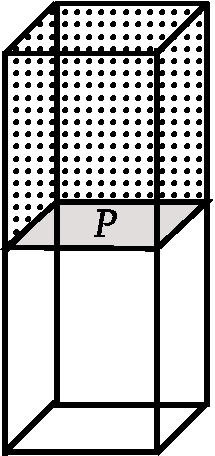
\includegraphics[height=6cm,width=3cm]{t353}
\end{figure}
\begin{tasks}(2)
	\task[\textbf{A.}] $T-\left(\frac{n a}{C_{V}}\right) \ln 2$
	\task[\textbf{B.}] $T+\left(\frac{n a}{C_{V}}\right) \ln 2$
	\task[\textbf{C.}]   $T-2 n\left(\frac{R T a}{C_{V}}\right)^{3 / 2}$
	\task[\textbf{D.}] $T+2 n\left(\frac{R T a}{C_{V}}\right)^{3 / 2}$
\end{tasks}
\begin{answer}
	
	So the correct answer is \textbf{option(A)}
\end{answer}
\begin{minipage}{\textwidth}
	\question A system is composed of a large number of non-interacting classical particles moving in two dimensions, which individually obey the Hamiltonian
	$$
	\frac{p_{x}^{2}+p_{y}^{2}}{2 m}+\frac{1}{2} m \omega^{2}\left(x^{2}+y^{2}\right)
	$$
	and the system is connected to a heat bath at a temperature $T$.
	The probability of finding a particle within a radius $R$ from the origin is given by
	\exyear{TIFR 2020}
\end{minipage}
\begin{tasks}(2)
	\task[\textbf{A.}] $1-\exp \left(-\frac{m \omega^{2} R^{2}}{2 T}\right)$
	\task[\textbf{B.}] $\exp \left(-\frac{m \omega^{2} R^{2}}{2 T}\right)$
	\task[\textbf{C.}] $\operatorname{erf}\left(\sqrt{\frac{m}{2 T}} \omega R\right)$
	\task[\textbf{D.}] $1-\frac{m \omega^{2} R^{2}}{2 T}$
\end{tasks}
\begin{answer}
	So the correct answer is \textbf{option(A)}
\end{answer}
\begin{minipage}{\textwidth}
	\question A particle of mass $m$ is confined inside a box with boundaries at $x=\pm L$. The ground state and the first excited state of this particle are $E_{1}$ and $E_{2}$ respectively.
	
	Now a repulsive delta function potential $\lambda \delta(x)$ is introduced at the centre of the box where the constant $\lambda$ satisfies
	$$
	0<\lambda \square \frac{1}{32 m}\left(\frac{h}{L}\right)^{2}
	$$
	If the energies of the new ground state and the new first excited state be denoted as $E_{1}^{\prime}$ and $E_{2}^{\prime}$ respectively, it follows that
	\exyear{TIFR 2020}
\end{minipage}
\begin{tasks}(2)
	\task[\textbf{A.}] $E_{1}^{\prime}>E_{1}, E_{2}^{\prime}>E_{2}$
	\task[\textbf{B.}] $E_{1}^{\prime}=E_{1}, E_{2}^{\prime}=E_{2}$
	\task[\textbf{C.}]   $E_{1}^{\prime}>E_{1}, E_{2}^{\prime}=E_{2}$
	\task[\textbf{D.}] $E_{1}^{\prime}=E_{1}, E_{2}^{\prime}>E_{2}$
\end{tasks}
\begin{answer}
	So the correct answer is \textbf{option(C)}
\end{answer}
\begin{minipage}{\textwidth}
	\question Three noninteracting particles whose masses are in the ratio $1: 4: 16$ are placed together in the same harmonic oscillator potential $V(x)$.
	
	The degeneracies of the first three energy eigenstates (ordered by increasing energy) will be
	\exyear{TIFR 2020}
\end{minipage}
\begin{tasks}(4)
	\task[\textbf{A.}] $1,1,1$
	\task[\textbf{B.}]   $1,1,2$
	\task[\textbf{C.}] $1,2,1$
	\task[\textbf{D.}] $1,2,2$
\end{tasks}
\begin{answer}
	So the correct answer is \textbf{option(B)}
\end{answer}
\begin{minipage}{\textwidth}
	\question The circuit shown represents a typical voltage-divider bias circuit for a transistor. Assume that resistance values and voltage values are typical for using the transistor as an amplifier.\\
	Which of the following changes in the circuit would result in an increase in the collector voltage $V_{C} ?$
	\exyear{TIFR 2020}
\end{minipage}
\begin{figure}[H]
	\centering
	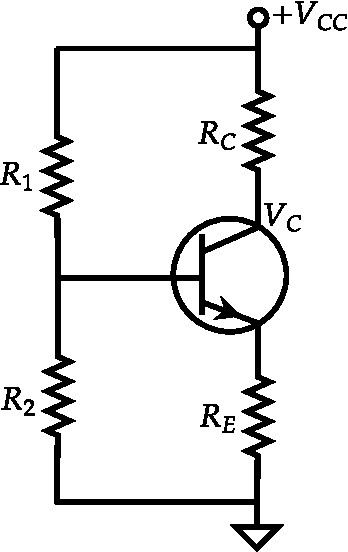
\includegraphics[height=6cm,width=3.5cm]{t354}
\end{figure}
\begin{tasks}(2)
	\task[\textbf{A.}]   $R_{2}$ is decreased slightly
	\task[\textbf{B.}]   $R_{2}$ is increased slightly
	\task[\textbf{C.}]   $R_{C}$ is decreased slightly
	\task[\textbf{D.}] $R_{C}$ is increased slightly
\end{tasks}
\begin{answer}
	So the correct answer is \textbf{option(A)}
\end{answer}
\begin{minipage}{\textwidth}
	\question A beam of $X$-rays is incident upon a powder sample of a material which forms simple cubic crystals of lattice constant $5.5 \AA^{\circ}$. The maximum wavelength of the $X$-rays which can produce diffraction from the planes with Miller indices $(0,0,5)$ is
	\exyear{TIFR 2020}
\end{minipage}
\begin{tasks}(4)
	\task[\textbf{A.}] $2.2$ \AA
	\task[\textbf{B.}] $55.0$ \AA
	\task[\textbf{C.}] $1.1 $\AA
	\task[\textbf{D.}] $27.5$ \AA
\end{tasks}
\begin{answer}
	$$
	d_{h k l}=\frac{a}{\sqrt{h^{2}+k^{2}+l^{2}}}=\frac{5.5}{5}=1.1 \AA
	$$
	
	According to Bragg's Law
	
	$$
	\begin{aligned}
	2 d \sin \theta &=n \lambda \\
	\lambda &=\frac{2 d \sin \theta}{n} \\
	\lambda_{\max } &=(2 d \sin \theta)_{\max }=2 d=2.2 \AA
	\end{aligned}
	$$
	So the correct answer is \textbf{option(A)}
\end{answer}
\begin{minipage}{\textwidth}
	\question Consider the nuclear decay chain of radio-Bismuth to Polonium to Lead, i.e.
	$$
	{ }_{83}^{219} \mathrm{Bi} \rightarrow_{84}^{210} \mathrm{Po} \rightarrow_{82}^{206} \mathrm{~Pb}
	$$
	where $\mathrm{Pb}-206\left({ }_{82}^{206} \mathrm{~Pb}\right)$ is a stable nucleus, and $\mathrm{Bi}-210\left({ }_{82}^{219} \mathrm{Bi}\right)$ and $\mathrm{Po}-206\left({ }_{84}^{210} \mathrm{Po}\right)$ are radioactive nuclei with half lives of about 5 days and 138 days respectively.
	
	If we start with a sample of pure $\mathrm{Bi}-210\left({ }_{82}^{219} \mathrm{Bi}\right)$, then a possible graph for the time evolution of the number of nuclei of these three species will be
	\exyear{TIFR 2020}
\end{minipage}
\begin{tasks}(2)
	\task[\textbf{A.}] \begin{figure}[H]
		\centering
		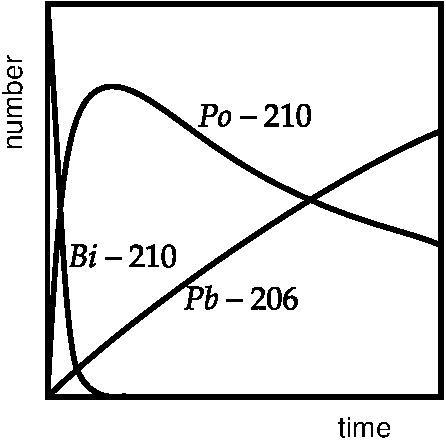
\includegraphics[height=4cm,width=4cm]{t355}
	\end{figure}
	\task[\textbf{B.}] \begin{figure}[H]
		\centering
		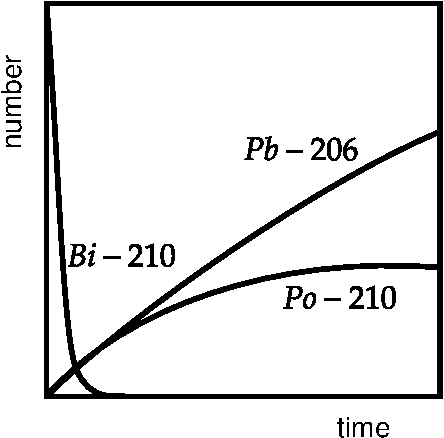
\includegraphics[height=4cm,width=4cm]{t356}
	\end{figure}
	\task[\textbf{C.}] \begin{figure}[H]
		\centering
		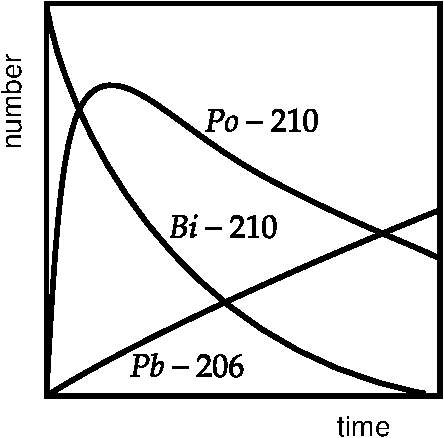
\includegraphics[height=4cm,width=4cm]{t357}
	\end{figure}
	\task[\textbf{D.}] \begin{figure}[H]
		\centering
		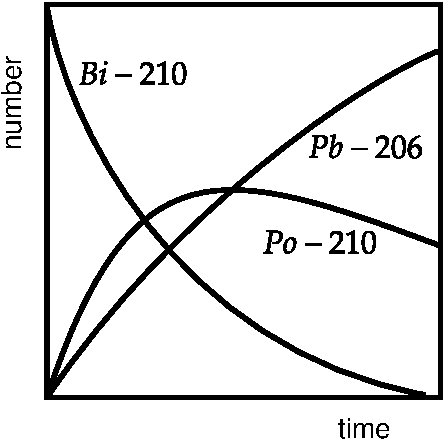
\includegraphics[height=4cm,width=4cm]{t358}
	\end{figure}
\end{tasks}
\begin{answer}
	Bi has very small half life compared to that of Po So, Bi will deccay very fast. The polonium will increasse from $\mathrm{O}$ and will get maximized and then it will fall. Lead will increase continuoulsy.\\
	So the correct answer is \textbf{option(B)}
\end{answer}
\begin{minipage}{\textwidth}
	\question A monochromatic laser beam is incident on a wet piece of filter paper atop a sheet of glass of thickness $d$. The pattern observed on the paper is shown in figure. If the radius of the inner ring observed is $R$, the refractive index of the glass must be
	\exyear{TIFR 2020}
\end{minipage}
\begin{figure}[H]
	\centering
	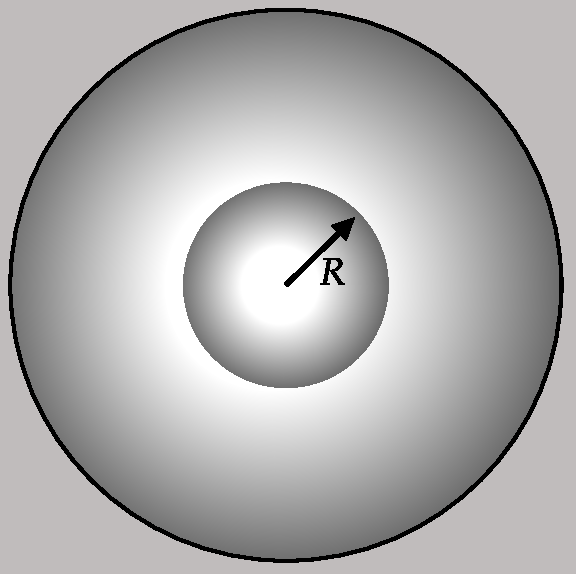
\includegraphics[height=4cm,width=4cm]{t359}
\end{figure}
\begin{tasks}(2)
	\task[\textbf{A.}] $\sin \left\{\tan ^{-1}\left(\frac{R}{2 d}\right)\right\}$
	\task[\textbf{B.}] $\sin \left\{\tan ^{-1}\left(\frac{R}{d}\right)\right\}$
	\task[\textbf{C.}] $\tan \left\{\sin ^{-1}\left(\frac{R}{2 d}\right)\right\}$
	\task[\textbf{D.}] $\tan \left\{\sin ^{-1}\left(\frac{R}{d}\right)\right\}$
\end{tasks}
\begin{answer}
	
	So the correct answer is \textbf{option(B)}
\end{answer}
\begin{minipage}{\textwidth}
	\question A plane polarised light wave with electric field expressed as
	$$
	\vec{E}(z, t)=E_{0} \hat{j} \cos (k z-\omega t)
	$$
	is incident from the left on the apparatus as sketched below.\\
	\begin{figure}[H]
		\centering
		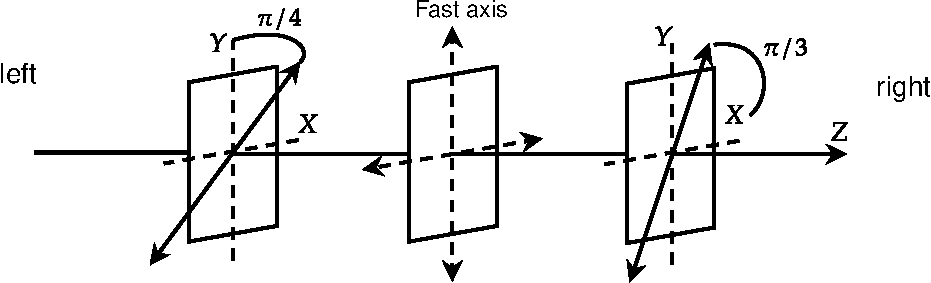
\includegraphics[height=3.5cm,width=11cm]{t360}
	\end{figure}
	The apparatus consists of (from left to right) a polariser with transmission axis at $\frac{\pi}{4}$ w.r.t. y-axis, followed by a quarter-wave plate with fast axis along the $y$-axis and finally, a polariser with transmission axis at $\frac{\pi}{3}$ about the $x$-axis.
	
	If the incident intensity of the wave is $I_{0}$, what will be intensity of the light emerging out of the apparatus (on the right)?
	\exyear{TIFR 2020}
\end{minipage}
\begin{tasks}(4)
	\task[\textbf{A.}]   $\frac{I_{0}}{4}$
	\task[\textbf{B.}] $\frac{I_{0}}{8}$
	\task[\textbf{C.}]   $\frac{3 I_{0}}{8}$
	\task[\textbf{D.}]   $\frac{I_{0}}{16}$
\end{tasks}
\begin{answer}$\left. \right. $\\
	\begin{figure}[H]
		\centering
		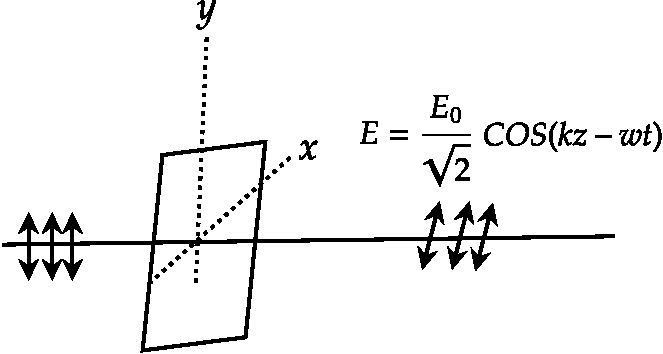
\includegraphics[height=3cm,width=5cm]{t 1f}
		\end{figure}
	After Polarizer, $E=\frac{E_{0}}{\sqrt{2}} \cos (k z-\omega t)$
	
	After quater wave plate, light will be circularly polarized
	$$
	\vec{E}=\frac{E_{0}}{2} \cos (k z-\omega t) \hat{i}+\frac{E_{0}}{2} \sin (k z-\omega t) \hat{j}
	$$
	After last polarizer,
	$$
	\begin{aligned}
	I &=\left(\frac{E_{0}}{2} \cos 60^{\circ}\right)^{2}+\left(\frac{E_{0}}{2} \cos 30^{\circ}\right)^{2} \\
	&=\frac{E_{0}^{2}}{4}\left(\frac{1}{4}+\frac{3}{4}\right)=\frac{E_{0}^{2}}{4}=\frac{I_{0}}{4}
	\end{aligned}
	$$\\
	So the correct answer is \textbf{option(A)}
\end{answer}
\begin{minipage}{\textwidth}
	\question The solution of the differential equation
	$$
	\frac{d y}{d x}=1+\frac{y}{x}-\frac{y^{2}}{x^{2}}
	$$
	for $x>0$ with the boundary condition $y=0$ at $x=1$. is given by $y(x)=$
	\exyear{TIFR 2020}
\end{minipage}
\begin{tasks}(4)
	\task[\textbf{A.}] $\frac{x\left(x^{2}-1\right)}{x^{2}+1}$
	\task[\textbf{B.}]   $\frac{x(x-1)}{x+1}$
	\task[\textbf{C.}]   $\frac{x-1}{x+1}$
	\task[\textbf{D.}] $\frac{x^{2}-1}{x^{2}+1}$
\end{tasks}
\begin{answer}
	
	So the correct answer is \textbf{option()}
\end{answer}
\begin{minipage}{\textwidth}
	\question The value of the integral
	$$
	\int_{0}^{\infty} \frac{d x}{x^{4}+4}
	$$
	is
	\exyear{TIFR 2020}
\end{minipage}
\begin{tasks}(4)
	\task[\textbf{A.}] $\frac{\pi}{8}$
	\task[\textbf{B.}] $\frac{3 \pi}{8}$
	\task[\textbf{C.}] $2 \pi$
	\task[\textbf{D.}] $\frac{\pi}{4}$
\end{tasks}
\begin{minipage}{\textwidth}
	\question A uniform rod of length $\ell$ and mass $m$ is suspended horizontally from a rigid support by two identical massless springs, each with stiffness constant $k$, as sketched below.\\
	\begin{figure}[H]
		\centering
		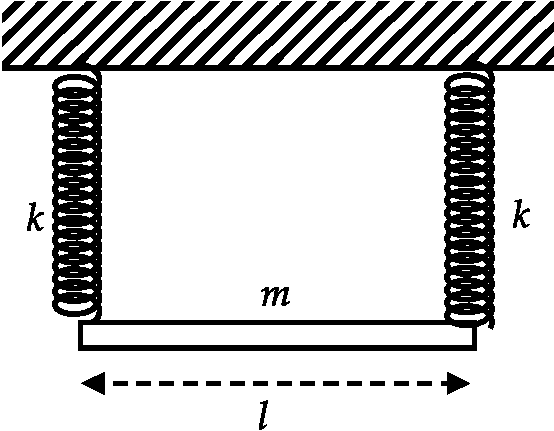
\includegraphics[height=3.5cm,width=4.5cm]{t361}
	\end{figure}
	If the springs can move only in the vertical direction, the frequency of small oscillations of the rod about equilibrium is given by
	\exyear{TIFR 2020}
\end{minipage}
\begin{tasks}(2)
	\task[\textbf{A.}]   $\sqrt{\frac{2 k}{m}}$ and $\sqrt{\frac{6 k}{m}}$
	\task[\textbf{B.}] $\sqrt{\frac{2 k}{m}}$ and $\sqrt{\frac{2 \pi k}{m}}$
	\task[\textbf{C.}] $\sqrt{\frac{\pi k}{2 m}}$ and $\sqrt{\frac{6 k}{m}}$
	\task[\textbf{D.}] $\sqrt{\frac{k}{m}}$ and $\sqrt{\frac{2 \pi k}{m}}$
\end{tasks}
\begin{minipage}{\textwidth}
	\question The Lagrangian of a system described by generalised coordinates $q_{1}$ and $q_{2}$ is given by
	$$
	L=\frac{a}{2}\left(\dot{q}_{1}^{2}+\dot{q}_{2}^{2}\right)-\frac{b^{2}}{\pi}\left(q_{1}^{2}+q_{2}^{2}\right)
	$$
	where $a$ and $b$ are constants. If follows that a conserved quantity in this system is
	\exyear{TIFR 2020}
\end{minipage}
\begin{tasks}(2)
	\task[\textbf{A.}] $q_{1} \dot{q}_{2}-q_{2} \dot{q}_{1}$
	\task[\textbf{B.}] $q_{1} \dot{q}_{2}+q_{2} \dot{q}_{1}$
	\task[\textbf{C.}] $\frac{q_{1} \dot{q}_{2}-q_{2} \dot{q}_{1}}{q_{1}^{2}+q_{2}^{2}}$
	\task[\textbf{D.}] $2 \pi\left(q_{1}^{2} \dot{q}_{2}+q_{2}^{2} \dot{q}_{1}\right)$
\end{tasks}
\begin{minipage}{\textwidth}
	\question Two conducting uncharged spheres of radii $R_{1}$ and $R_{2}$ are connected by an infinitesimally thin wire. The centres of the spheres are located at $\bar{r}_{1}$ and $\vec{r}_{2}$ respectively with respect to the origin $O$. The system is subjected to an uniform external electric field $\vec{E}_{0}$.\\
	\begin{figure}[H]
		\centering
		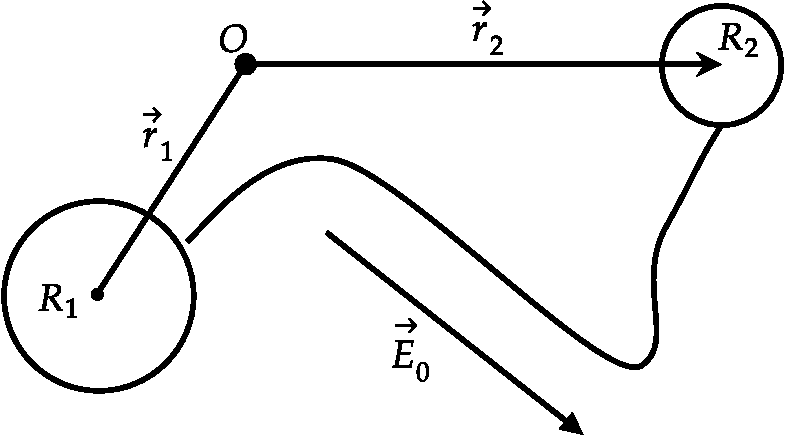
\includegraphics[height=3cm,width=5.5cm]{t362}
	\end{figure}
	If the wire cannot support a net charge and two spheres are separated by distance much larger than the radii of each of them, the induced dipole moment in the system would be
	\exyear{TIFR 2020}
\end{minipage}
\begin{tasks}(2)
	\task[\textbf{A.}] $4 \pi \epsilon_{0} \frac{R_{1} R_{2}}{R_{1}+R_{2}}\left\{\vec{E}_{0} .\left(\vec{r}_{2}-\vec{r}_{1}\right)\right\}\left(\vec{r}_{2}-\vec{r}_{1}\right)$
	\task[\textbf{B.}] $\frac{1}{4 \pi \epsilon_{0}} \frac{R_{1} R_{2}}{\left(R_{1}+R_{2}\right)}\left\{\vec{E}_{0} \cdot\left(\vec{r}_{2}-\vec{r}_{1}\right)\right\}\left(\vec{r}_{2}-\vec{r}_{1}\right)$
	\task[\textbf{C.}] $4 \pi \epsilon_{0} \frac{R_{1}+R_{2}}{R_{1} R_{2}}\left\{\vec{E}_{0} \cdot\left(\vec{r}_{2}-\vec{r}_{1}\right)\right\}\left(\vec{r}_{2}-\vec{r}_{1}\right)$
	\task[\textbf{D.}] Zero
\end{tasks}
\begin{minipage}{\textwidth}
	\question Consider the following situation.
	An infinite plane metallic plate of thickness $1.8 \mathrm{~cm}$ is placed along the $x-y$ plane, with $z$ axis normal to the sheet (see figure).\\
	\begin{figure}[H]
		\centering
		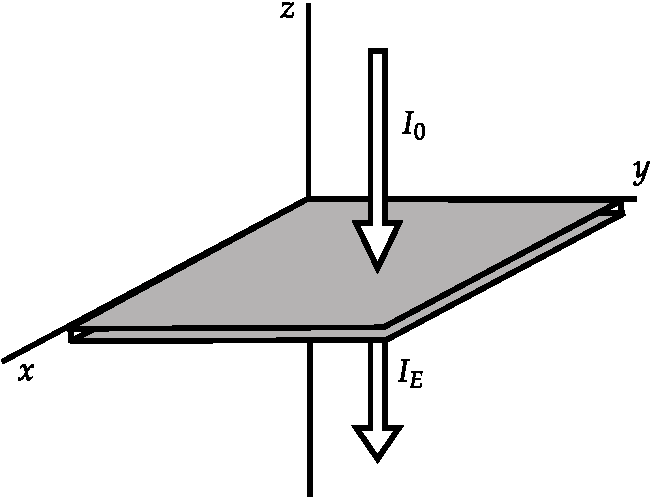
\includegraphics[height=4.5cm,width=5.5cm]{t363}
	\end{figure}
	A plane radio wave of intensity $I_{0}$ and frequency $29.5 \mathrm{MHz}$ propagates in vacuum along the negative $z$-axis and strikes the metal foil at normal incidence.
	If the metal of the foil has conductivity $5.9 \Omega^{-1} m^{-1}$ and magnetic permeability $\mu \square 1$, the intensity $I_{E}$ of the emergent wave will be approximately
	\exyear{TIFR 2020}
\end{minipage}
\begin{tasks}(4)
	\task[\textbf{A.}]   $0.26 I_{0}$
	\task[\textbf{B.}] $0.51 I_{0}$
	\task[\textbf{C.}] $0.29 \times 10^{-7} I_{0}$
	\task[\textbf{D.}] $2.08 \times 10^{-4} I_{0}$
\end{tasks}
\begin{minipage}{\textwidth}
	\question In a certain atom, the ground state and first excited state of the valence electron are $-7.8 \mathrm{eV}$ and $-3.9 \mathrm{eV}$, while all the higher exited states have energies very close to zero. The ground state has a degeneracy of 2 , while the first excited state has a degeneracy of 6 . It follows that if these atoms reside in the outer layers of a blue giant star at a temperature around $2.32 \times 10^{4} K$, the average per atom will be approximately
	\exyear{TIFR 2020}
\end{minipage}
\begin{tasks}(2)
	\task[\textbf{A.}] $-5.1 \mathrm{eV}$
	\task[\textbf{B.}] $-5.9 \mathrm{eV}$
	\task[\textbf{C.}]   $-6.8 \mathrm{eV}$
	\task[\textbf{D.}] $-4.4 \mathrm{eV}$
\end{tasks}
\begin{minipage}{\textwidth}
	\question A square lattice consists $2 N$ sites, of which alternate sites are labelled $A$ and $B .$ An example with $N=6$ is shown on the right. Now, $N$ identical classical particles are distributed over these sites, such that each site can accommodate at most one particle.
	The fraction of the total number $N$ of particles occupying $A$ sites is denoted $\alpha$ and the fraction occupying $B$ sites is denoted $\beta$,so that $\alpha+\beta=1$. If $\alpha, \beta$ are fixed and $N \square 1$, the entropy $S$ of the system can be written 
	\exyear{TIFR 2020}
\end{minipage}
\begin{figure}[H]
	\centering
	
\includegraphics[height=5cm,width=5cm]{t364}
\end{figure}
\begin{tasks}(2)
	\task[\textbf{A.}]   $S=-2 N k_{B} T(\alpha \ln \alpha+\beta \ln \beta)$
	\task[\textbf{B.}] $S=2 N k_{B} T(\alpha \ln \alpha+\beta \ln \beta)$
	\task[\textbf{C.}]   $S=-2 N k_{B} T(\alpha \ln \alpha-\beta \ln \beta)$
	\task[\textbf{D.}]   $S=2 N k_{B} T(\alpha \ln \alpha-\beta \ln \beta)$
\end{tasks}
\begin{minipage}{\textwidth}
	\question A particle of mass $m$ is placed in one dimensional harmonic oscillator potential
	$$
	V(x)=\frac{1}{2} m \omega^{2} x^{2}
	$$
	At $t=0$, its wavefunction is $\psi(x)$. At $t=2 \pi / \omega$ its wavefunction will be
	\exyear{TIFR 2020}
\end{minipage}
\begin{tasks}(4)
	\task[\textbf{A.}]   $\psi(x)$
	\task[\textbf{B.}] $-\psi(x)$
	\task[\textbf{C.}]   $-\pi \psi(x)$
	\task[\textbf{D.}] $\frac{2 \pi}{\omega} \psi(x)$
\end{tasks}
\begin{minipage}{\textwidth}
	\question A spin- 2 nucleus absorbs a spin- $1 / 2$ electron and is then observed to decay to a stable nucleus in two stages, recoiling against an emitted invisible particle in the first stage and against an emitted spin-1 photon in the second stage. If the stable nucleus is spinless, then the spin of the invisible particle is
	\exyear{TIFR 2020}
\end{minipage}
\begin{tasks}(4)
	\task[\textbf{A.}] $\frac{3}{2}$ or $\frac{5}{2}$
	\task[\textbf{B.}] $\frac{3}{2}$
	\task[\textbf{C.}] $\frac{1}{2}$ or $\frac{3}{2}$
	\task[\textbf{D.}] $\frac{1}{2}$
\end{tasks}
\begin{minipage}{\textwidth}
	\question The circuit sketched below is called a relaxation oscillator.\\
	\begin{figure}[H]
		\centering
		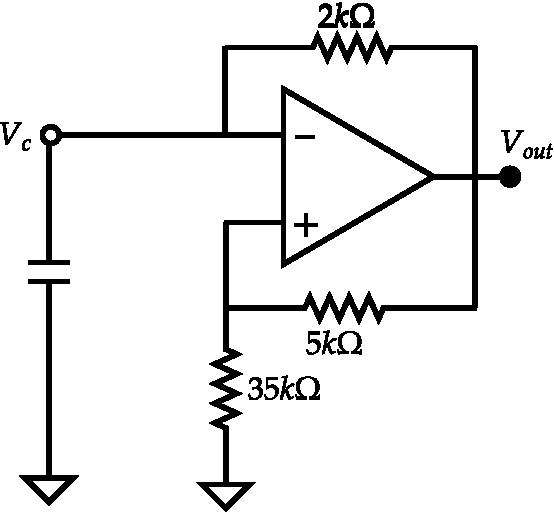
\includegraphics[height=4.5cm,width=5cm]{t365}
	\end{figure}
	For the parameters indicated in the figure, the ratio of the maximum voltage at $V_{\text {out }}$ to the maximum voltage at $V_{C}$ is
	\exyear{TIFR 2020}
\end{minipage}
\begin{tasks}(4)
	\task[\textbf{A.}] $\frac{1}{8}$
	\task[\textbf{B.}] $\frac{1}{7}$
	\task[\textbf{C.}] $\frac{2}{7}$
	\task[\textbf{D.}] $\frac{1}{4}$
\end{tasks}
\begin{minipage}{\textwidth}
	\question The figure below shows a carrier frequency $4 \mathrm{kHz}$ being amplitude-modulated by a sine wave-signal.\\
	\begin{figure}[H]
		\centering
		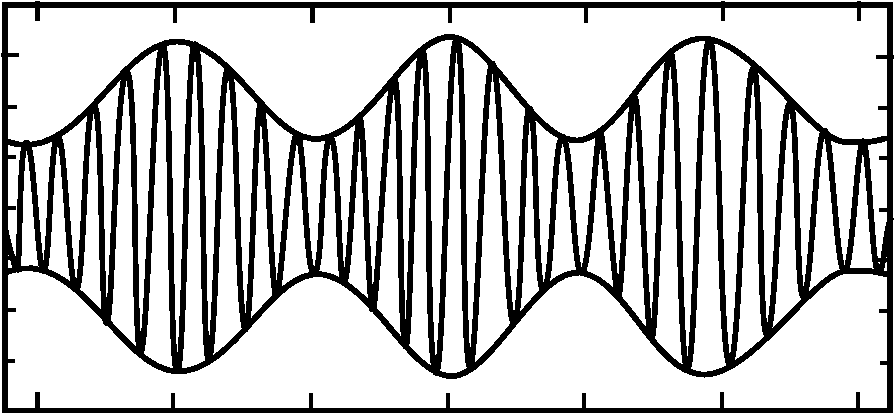
\includegraphics[height=3cm,width=6cm]{t366}
	\end{figure}
	In order to transmit the signal (without distortion) the minimum bandwidth needed would be
	\exyear{TIFR 2020}
\end{minipage}
\begin{tasks}(4)
	\task[\textbf{A.}] $8 \mathrm{kHz}$
	\task[\textbf{B.}]   $2 \mathrm{kHz}$
	\task[\textbf{C.}]   $4 \mathrm{kHz}$
	\task[\textbf{D.}]   $6 \mathrm{kHz}$
\end{tasks}
\begin{minipage}{\textwidth}
	\question A semiconductor with donor impurities can be thought in terms of a filled valence band, a filled donor level and an empty valence band at $T=0$, as shown in the figure below \\
	\begin{figure}[H]
		\centering
		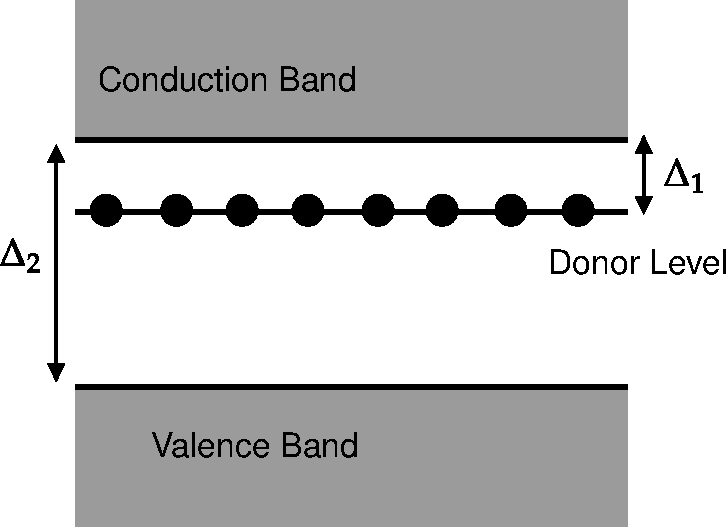
\includegraphics[height=3cm,width=5cm]{t367}
	\end{figure}
	If the band gap between donor level and conduction band is $\Delta_{1}$ and that between conduction and valence band is $\Delta_{2}$ where $\Delta_{2} \square \Delta_{1}$, which of the following figures depict the qualitative features of the resistance $(R)$ - vs-temperature $(T)$ graph of the semiconductor?
	(Assume temperature-independent scattering rates and a flat density of states for the bands.)
	\exyear{TIFR 2020}
\end{minipage}
\begin{tasks}(2)
	\task[\textbf{A.}] \begin{figure}[H]
		\centering
		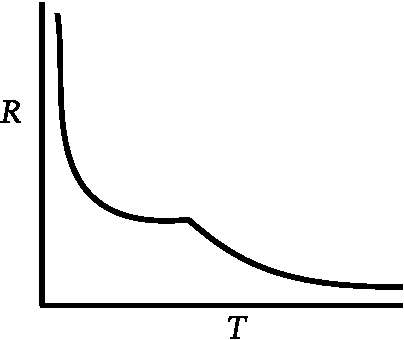
\includegraphics[height=4cm,width=4.5cm]{t368}
	\end{figure}
	\task[\textbf{B.}] \begin{figure}[H]
		\centering
		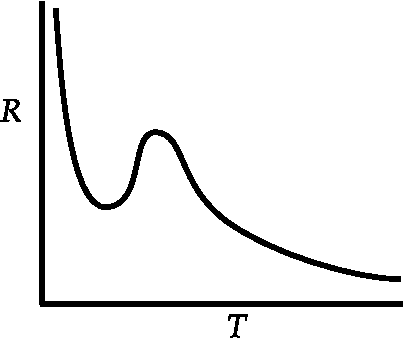
\includegraphics[height=4cm,width=4.5cm]{t369}
	\end{figure}
	\task[\textbf{C.}] \begin{figure}[H]
		\centering
		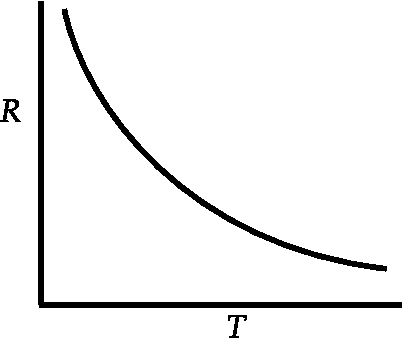
\includegraphics[height=4cm,width=4.5cm]{t370}
	\end{figure}
	\task[\textbf{D.}] \begin{figure}[H]
		\centering
		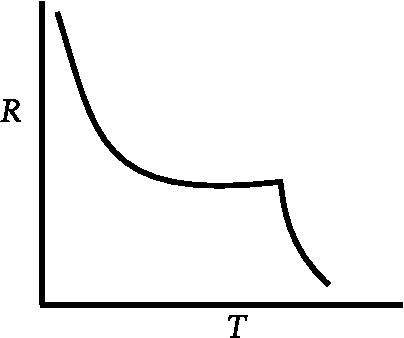
\includegraphics[height=4cm,width=4.5cm]{t371}
	\end{figure}
\end{tasks}
\begin{minipage}{\textwidth}
	\question Two atomic nuclei $A$ and $B$ have masses such that $m(B)=2 m(A)$, in the laboratory frame, the nucleus $B$ is kept stationary, while the nucleus $A$ is given a kinetic energy $300 \mathrm{MeV}$ and a made to collide with $B$. It is found that the two nuclei fuse to form a compound nucleus $C$.\\
	If the $Q$-value of the reaction is $-30 \mathrm{MeV}$, the excitation energy of the compound nucleus can be estimated as
	\exyear{TIFR 2020}
\end{minipage}
\begin{tasks}(4)
	\task[\textbf{A.}] $81 \mathrm{MeV}$
	\task[\textbf{B.}]   $170 \mathrm{MeV}$
	\task[\textbf{C.}]   $330 \mathrm{MeV}$
	\task[\textbf{D.}] $270 \mathrm{MeV}$
\end{tasks}
\begin{minipage}{\textwidth}
	\question Which of the following decays is forbidden?
	\exyear{TIFR 2020}
\end{minipage}
\begin{tasks}(2)
	\task[\textbf{A.}]   $\pi^{0} \rightarrow \gamma+\gamma$
	\task[\textbf{B.}] $K^{0} \rightarrow \pi^{+}+\pi^{-}+\pi^{0}$
	\task[\textbf{C.}] $\mu^{-} \rightarrow e^{-}+v_{e}+\bar{v}_{\mu}$
	\task[\textbf{D.}] $n^{0} \rightarrow p^{+}+e^{-}+\bar{v}_{e}$
\end{tasks}
\end{questions}
\begin{abox}
	TIFR-2019
\end{abox}
\begin{questions}
\begin{minipage}{\textwidth}
	\question Consider the surface defined by $a x^{2}+b y^{2}+c z+d=0$, where $a, b, c$ and $d$ are constants. If $\hat{n}_{1}$ and $\hat{n}_{2}$ are unit normal vectors to the surface at the points $(x, y, z)=(1,1,0)$ and $(0,0,1)$ respectively and $\hat{m}$ is a unit vector normal to both $\hat{n}_{1}$ and $\hat{n}_{2}$, then $\hat{m}=$
	\exyear{TIFR 2019}
\end{minipage}
\begin{tasks}(4)
	\task[\textbf{A.}] $\frac{-a i+b j}{\sqrt{a^{2}+b^{2}}}$
	\task[\textbf{B.}] $\frac{b \hat{i}-a \hat{j}}{\sqrt{a^{2}+b^{2}}}$
	\task[\textbf{C.}] $\frac{2 a \hat{i}+2 b \hat{j}-c \hat{k}}{\sqrt{4 a^{2}+4 b^{2}+c^{2}}}$
	\task[\textbf{D.}] $\frac{a \hat{i}+b \hat{j}-c \hat{k}}{\sqrt{a^{2}+b^{2}+c^{2}}}$
\end{tasks}
\begin{answer}
	Equation of surface is given by
	$$
	\begin{aligned}
	S & \equiv a x^{2}+b y^{2}+c z+d=0 \\
	\nabla S &=2 a \hat{i}+2 b \hat{j}+c \hat{k} \\
	\left.\nabla S\right|_{(1,1,0)} &=2 a \hat{i}+2 b \hat{j}+c \hat{k} \\
	\left.\nabla S\right|_{(0,0,1)} &=c \hat{k} \\
	\hat{n}_{1} &=\frac{\nabla S}{|\nabla S|}=\frac{2 a \hat{i}+2 b \hat{j}+c \hat{k}}{\sqrt{4 a^{2}+4 b^{2}+c^{2}}} \\
	\hat{n}_{2} &=\frac{\nabla S}{|\nabla S|}=\hat{k}
	\end{aligned}
	$$
	Unit vector $\hat{m}$ will lie in direction of $\hat{n}_{1} \times \hat{n}_{2}$
	$$
	\begin{aligned}
	\hat{n}_{1} \times \hat{n}_{2} &=\frac{2 a \hat{i}+2 b \hat{j}+c \hat{k}}{\sqrt{4 a^{2}+4 b^{2}+c^{2}}} \times \hat{k} \\
	&=\frac{-2 a \hat{j}+2 b \hat{i}}{\sqrt{4 a^{2}+4 b^{2}+c^{2}}}
	\end{aligned}
	$$
	Unit vector along $\hat{n}_{1} \times \hat{n}_{2}$,
	$$
	\hat{m}=\frac{b \hat{i}-a \hat{j}}{\sqrt{a^{2}+b^{2}}}
	$$
	So the correct answer is \textbf{option(B)}
\end{answer}
\begin{minipage}{\textwidth}
	\question The eigenvalues of a $3 \times 3$ matrix $M$ are
	$$
	\lambda_{1}=2 \quad \lambda_{2}=-1 \quad \lambda_{3}=1
	$$
	and the eigenvectors are
	$$
	e_{1}=\left(\begin{array}{l}
	1 \\
	1 \\
	1
	\end{array}\right) \quad e_{2}=\left(\begin{array}{c}
	1 \\
	1 \\
	-2
	\end{array}\right) \quad e_{3}=\left(\begin{array}{c}
	1 \\
	-1 \\
	0
	\end{array}\right)
	$$
	The matrix $M$ is
	\exyear{TIFR 2019}
\end{minipage}
\begin{tasks}(2)
	\task[\textbf{A.}] $\left(\begin{array}{lll}1 & 0 & 1 \\ 0 & 1 & 1 \\ 1 & 1 & 0\end{array}\right)$
	\task[\textbf{B.}]   $\left(\begin{array}{lll}0 & 1 & 1 \\ 1 & 0 & 0 \\ 1 & 0 & 2\end{array}\right)$
	\task[\textbf{C.}] $\left(\begin{array}{ccc}1 & 0 & 0 \\ 1 & 0 & -1 \\ 0 & -1 & 1\end{array}\right)$
	\task[\textbf{D.}] $\left(\begin{array}{lll}1 & 1 & 0 \\ 1 & 0 & 1 \\ 0 & 1 & 1\end{array}\right)$
\end{tasks}
\begin{answer}
	$\hat{e}_{1}=\left[\begin{array}{l}1 \\ 1 \\ 1\end{array}\right]$ is not eigenvectors of matrix in (b) \& (c).\\
	$\hat{e}_{3}=\left[\begin{array}{c}1 \\ -1 \\ 0\end{array}\right]$ is not eigenvector of matrix in (d).\\
	So, only option left is (a) and we can clearly verify that $\hat{e}_{1}, \hat{e}_{2}$ and $\hat{e}_{3}$ are eigenvector of matrix in (a).\\
	So the correct answer is \textbf{option(A)}
\end{answer}
\begin{minipage}{\textwidth}
	\question Which of the following operations will transform a tetrahedron $A B C D$ with vertices as listed below\\
	$\begin{array}{lllll} & x & y & z \\ A & 0 & 0 & 0 \\ B & 1 & 0 & 0 \\ C & 0 & 1 & 0 \\ D & 0 & 0 & 2\end{array}$\\
	\begin{figure}[H]
		\centering
		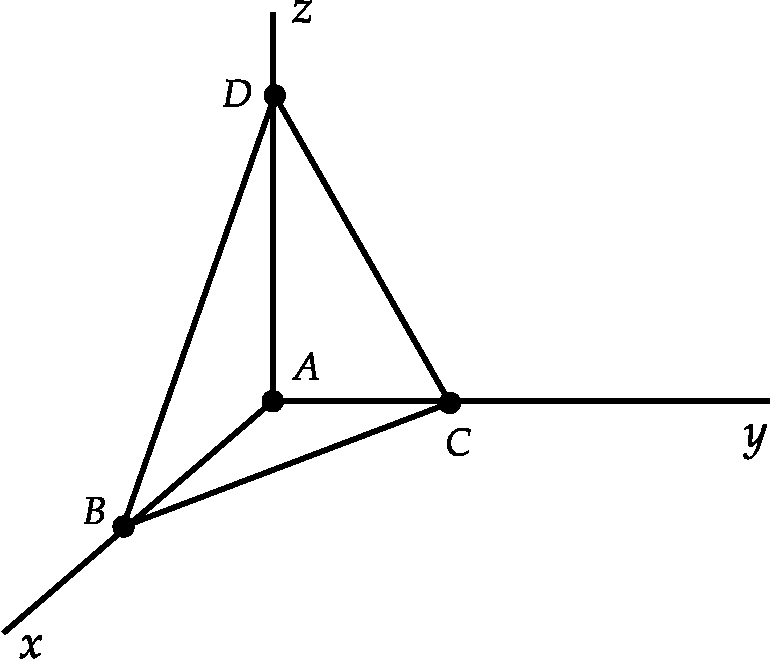
\includegraphics[height=4.5cm,width=5cm]{t286}
	\end{figure}
	Into a tetrahedron $A B C D$ with vertices as listed below\\
	$\begin{array}{cccc} & x & y & z \\ A & 0 & 0 & 0 \\ B & 0 & 1 & 0 \\ C & 0 & 0 & 1 \\ D & 2 & 0 & 0\end{array}$\\
	\begin{figure}[H]
		\centering
		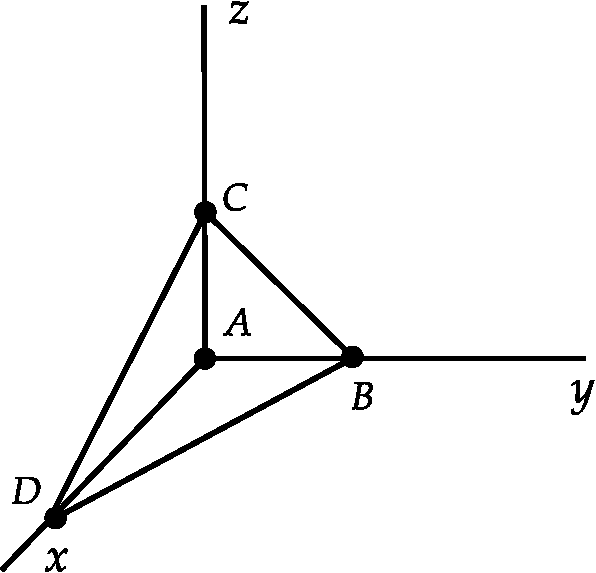
\includegraphics[height=3.5cm,width=4.5cm]{t287}
	\end{figure}
	Up to suitable translation?
	\exyear{TIFR 2019}
\end{minipage}
\begin{tasks}(1)
	\task[\textbf{A.}]   A rotation about $x$ axis by $\frac{\pi}{2}$ then a rotation about $z$ axis by $\frac{\pi}{2}$
	\task[\textbf{B.}]   A reflection in the $x y$ plane, then a rotation about $x$ axis by $\frac{\pi}{2}$
	\task[\textbf{C.}] A reflection in the $y z$ plane, then a rotation about $x y$ plane
	\task[\textbf{D.}] A rotation about $y$ axis by $\frac{\pi}{2}$, then a reflection in the $x z$ plane
\end{tasks}
\begin{answer}
	So the correct answer is \textbf{option(A)}
\end{answer}
\begin{minipage}{\textwidth}
	\question A British coin has a portrait of Queen Elizabeth II on the 'heads' side and 'ONE POUND' written on the tails side, while an Indian coin has a portrait of Mahatma Gandhi on the heads side and ' 10 RUPEES' written on the 'tails' side (see below).\\
	These two coins are tossed simultaneously twice in succession.
	The result of the first toss was 'heads' for both the coins. The probability that the result of the second toss had a ' 10 RUPEES' side is
	\exyear{TIFR 2019}
\end{minipage}
\begin{tasks}(4)
	\task[\textbf{A.}]   $\frac{1}{2}$
	\task[\textbf{B.}]   $\frac{4}{7}$
	\task[\textbf{C.}]   $\frac{3}{5}$
	\task[\textbf{D.}]   $\frac{2}{3}$
\end{tasks}
\begin{answer}
	So the correct answer is \textbf{option(B)}
\end{answer}
\begin{minipage}{\textwidth}
	\question A set of polynomials of order $n$ are given by the formula
	$$
	p_{n}(x)=(-1)^{n} \exp \left(\frac{x^{2}}{2}\right) \frac{d^{n}}{d x^{n}} \exp \left(-\frac{x^{2}}{2}\right)
	$$
	The polynomial $p_{7}(x)$ of order $n=7$ is
	\exyear{TIFR 2019}
\end{minipage}
\begin{tasks}(1)
	\task[\textbf{A.}] $x^{7}-21 x^{5}+105 x^{4}+35 x^{3}-105 x$
	\task[\textbf{B.}]   $x^{6}-21 x^{5}+105 x^{4}-105 x^{3}+21 x^{2}+x$
	\task[\textbf{C.}] $x^{7}-21 x^{5}+105 x^{3}-105 x+21$
	\task[\textbf{D.}] $x^{7}-21 x^{5}+105 x^{3}-105 x$
\end{tasks}
\begin{answer}
	$P_{n}(x)$ is basically Hermite polynomial which is even if $n$ is even and odd when $n$ is odd. Making use of this property we can clearly see that (a), (b), (c) are not Hermite polynomial. So (d) is only correct answer.\\
	So the correct answer is \textbf{option(D)}
\end{answer}
\begin{minipage}{\textwidth}
	\question A particle of mass $m$ is placed on an inclined plane making an adjustable angle $\theta$ with the horizontal, as shown in the figure. The coefficient of friction between the particle and the inclined plane is $\mu$.\\
	If the inclined plane is moving horizontally with a uniform acceleration $a<\frac{g}{\mu}$ (see figure), the value of $\theta$ for which the particle will remain at rest on the plane is
	\exyear{TIFR 2019}
\end{minipage}
\begin{figure}[H]
	\centering
	\includegraphics[height=2.5cm,width=3cm]{t288}
\end{figure}
\begin{tasks}(2)
	\task[\textbf{A.}]   $\theta=\tan ^{-1}\left(\frac{\mu g+a}{g+\mu a}\right)$
	\task[\textbf{B.}] $\theta=-\cot ^{-1}\left(\frac{\mu a+g}{a+\mu g}\right)$
	\task[\textbf{C.}] $\theta=\tan ^{-1}\left(\frac{\mu g+a}{g-\mu a}\right)$
	\task[\textbf{D.}] $\theta=\cot ^{-1}\left(\frac{\mu a-g}{a+\mu g}\right)$
\end{tasks}
\begin{answer}Taking observer attached with inclined plate
	\begin{figure}[H]
		\centering
		\includegraphics[height=3cm,width=5cm]{t1h}
		$$
		\begin{aligned}
		F_{x} &=0 \\
		\Rightarrow \quad N \sin \theta-m a-\mu N \cos \theta &=0 \\
		\Rightarrow \quad & N &=\frac{m g}{\mu \sin \theta+\cos \theta}
		\end{aligned}
		$$
		Putting $N$ in (1)
		$\begin{aligned}(\sin \theta-\mu \cos \theta) \frac{m g}{\mu \sin \theta+\cos \theta} &=m a \\ \Rightarrow \quad \frac{(\tan \theta-\mu) g}{(\mu \tan \theta+1)} &=a \\ \Rightarrow \quad g \tan \theta-\mu g &=a \mu \tan \theta+a \\ \Rightarrow \quad(g-a \mu) \tan \theta &=a+\mu g \\ \tan \theta &=\frac{a+\mu g}{g-a \mu} \\ \text { So, } \quad \theta &=\tan ^{-1}\left[\frac{a+\mu g}{g-a \mu}\right] \end{aligned}$
	\end{figure}
	So the correct answer is \textbf{option(C)}
\end{answer}
\begin{minipage}{\textwidth}
	\question Two bodies $A$ and $B$ of equal mass are suspended from two rigid supports by separate massless springs having spring constants $k_{1}$ and $k_{2}$ respectively. If the bodies oscillate vertically such that their maximum velocities are equal the ratio of the amplitude of oscillations of $A$ to that of $B$ is
	\exyear{TIFR 2019}
\end{minipage}
\begin{figure}[H]
	\centering
	\includegraphics[height=3cm,width=4cm]{t289}
\end{figure}
\begin{tasks}(4)
	\task[\textbf{A.}] $\frac{k_{2}}{k_{1}}$
	\task[\textbf{B.}] $\frac{k_{2}}{k_{1}}$
	\task[\textbf{C.}] $\sqrt{\frac{k_{1}}{k_{2}}}$
	\task[\textbf{D.}] $\sqrt{\frac{k_{2}}{k_{1}}}$
\end{tasks}
\begin{answer}
	Equation of motion of $A$ and $B$ are given by
	$$
	\begin{aligned}
	&y_{1}=a_{1} \sin \omega_{1} t \\
	&y_{2}=a_{2} \sin \omega_{2} t \\
	&\omega_{1}=\sqrt{\frac{k_{1}}{m}} \\
	&\omega_{2}=\sqrt{\frac{k_{2}}{m}}
	\end{aligned}
	$$
	where
	Their velocities are given by
	$$
	\begin{gathered}
	v_{1}=\frac{d y_{1}}{d t}=a_{1} \omega_{1} \cos \omega_{1} t \\
	v_{2}=\frac{d y_{2}}{d t}=a_{2} \omega_{2} \cos \omega_{2} t \\
	v_{\operatorname{lmax}}=v_{2 \max }
	\end{gathered}
	$$
	Now,\\
	$\Rightarrow a_{1} \omega_{1}=a_{2} \omega_{2}$\\
	$\Rightarrow \quad a_{1} \sqrt{\frac{k_{1}}{m}}=a_{2} \sqrt{\frac{k_{2}}{m}} \Rightarrow \frac{a_{1}}{a_{2}}=\sqrt{\frac{k_{2}}{k_{1}}}$\\
	So the correct answer is \textbf{option(D)}
\end{answer}
\begin{minipage}{\textwidth}
	\question A particle of mass $m$ is bounced on the ground with a velocity $u$ making an angle of $\theta$ with the ground. The coefficient of restitution for collisions between the particle and the ground is $\varepsilon$ and frictional effects are negligible both on the ground and in the air. The horizontal distance travelled by the particle from the point of initial impact till it begins to slide along the ground is
	\exyear{TIFR 2019}
\end{minipage}
\begin{figure}[H]
	\centering
	\includegraphics[height=2cm,width=5cm]{t290}
\end{figure}
\begin{tasks}(2)
	\task[\textbf{A.}] $\frac{u^{2}}{2 g}\left(\frac{\varepsilon}{1-\varepsilon}\right) \sin 2 \theta$
	\task[\textbf{B.}] $\frac{u^{2}}{g}\left(\frac{1}{1-\varepsilon}\right) \sin \theta$
	\task[\textbf{C.}] $\frac{u^{2}}{g}\left(\frac{\varepsilon}{1-\varepsilon}\right) \tan 2 \theta$
	\task[\textbf{D.}] $\frac{u^{2}}{g}\left(\frac{\varepsilon}{1-\varepsilon}\right) \sin 2 \theta$
\end{tasks}
\begin{answer}
	\begin{figure}[H]
		\centering
		\includegraphics[height=3cm,width=5cm]{t1i}\\
	Conserving linear momentum along $x$-axis.
	$$
	\begin{aligned}
	m u^{\prime} \cos \theta^{\prime} &=m u \cos \theta \\
	e=\frac{v_{2}^{\prime}-v_{1}^{\prime}}{v_{1}-v_{2}} &=\frac{u^{\prime} \sin \theta^{\prime}-0}{0-(u \sin \theta)} \\
	u^{\prime} \sin \theta^{\prime} &=e u \sin \theta
	\end{aligned}
	$$
	$$
	\Rightarrow
	$$
	Now,
	$$
	\begin{aligned}
	R_{1} &=u^{\prime} \cos \theta^{\prime} \cdot \frac{2 u^{\prime} \sin \theta^{\prime}}{g} \\
	&=u \cos \theta \cdot \frac{2 u \sin \theta}{g}=\frac{e u^{2} \sin 2 \theta}{g}
	\end{aligned}
	$$
	Similarly,
	So,
	$$
	\begin{aligned}
	R_{2} &=\frac{e^{2} u^{2} \sin 2 \theta}{g} \\
	R_{3} &=\frac{e^{3} u^{2} \sin 2 \theta}{g} \\
	\vdots & \\
	R &=R_{1}+R_{2}+R_{3}+\ldots \\
	&=\frac{u^{2} \sin 2 \theta}{g}\left[e+e^{2}+e^{3}+\ldots\right] \\
	&=\frac{u^{2}}{g}\left(\frac{e}{1-e}\right) \sin 2 \theta
	\end{aligned}
	$$
	\end{figure}
	So the correct answer is \textbf{option(D)}
\end{answer}
\begin{minipage}{\textwidth}
	\question The three-dimensional object sketch on the right is made by taking a solid sphere of uniform density (shaded) with radius $R$, and scooping out a spherical cavity (unshaded) as shown, which has diameter $R$.
	In this object has mass $M$, its moment of inertia about the tangential axis passing through the point where the spheres tough (as shown in the figure) is
	\exyear{TIFR 2019}
\end{minipage}
\begin{figure}[H]
	\centering
	\includegraphics[height=3cm,width=3.2cm]{t291}
\end{figure}
\begin{tasks}(4)
	\task[\textbf{A.}]   $\frac{3}{16} M R^{2}$
	\task[\textbf{B.}] $\frac{62}{35} M R^{2}$
	\task[\textbf{C.}] $\frac{31}{70} M R^{2}$
	\task[\textbf{D.}] $\frac{31}{20} M R^{2}$
\end{tasks}
\begin{answer}
	MI of solid sphere about tangential axis is
	\begin{figure}[H]
		\centering
		\includegraphics[height=3cm,width=4cm]{t 1k}
	$$
	\begin{aligned}
	I &=I_{\mathrm{cm}}+M R^{2} \\
	&=\frac{2}{5} M R^{2}+M R^{2}=\frac{7}{5} M R^{2} \\
	M &=\rho\left[\frac{4}{3} \pi R^{3}-\frac{4}{3} \pi\left(\frac{R}{2}\right)^{3}\right] \\
	&=\rho \frac{4}{3} \pi R^{3} \frac{7}{8}=\frac{7}{6} \rho \pi R^{3} \\
	\rho &=\frac{6 M}{7 \pi R^{3}}
	\end{aligned}
	$$
	Given mass distribution can be seen as superposition of two mass distribution
	\begin{figure}[H]
		\centering
		\includegraphics[height=3cm,width=5cm]{t 1j}
	\end{figure}
	\end{figure}
So,
$$
\begin{aligned}
I &=I_{1}+I_{2} \\
&=\frac{7}{5}\left(\rho \frac{4}{3} \pi R^{3}\right) R^{2}+\frac{7}{5}\left(-\rho \cdot \frac{4}{3} \pi\left(\frac{R}{2}\right)^{3}\right)\left(\frac{R}{2}\right)^{2} \\
&=\frac{7}{5} \cdot \rho \frac{4}{3} \pi R^{5}\left(1-\frac{1}{32}\right)
\end{aligned}
$$\\
$=\frac{28}{15} \times \frac{31}{32} \cdot \rho \pi R^{5}$\\
$=\frac{28}{15} \times \frac{31}{32} \times \frac{6 M}{7 \pi R^{3}} \pi R^{5}=\frac{31}{20} M R^{2}$\\
	So the correct answer is \textbf{option(D)}
\end{answer}
\begin{minipage}{\textwidth}
	\question Consider three straight coplanar, parallel wires of infinite length where the distance between adjacent where is $d$. Each wire carries a current $I$ in the same direction. The perpendicular distance from the middle wire (on either side) where the magnetic field vanishes is
	\exyear{TIFR 2019}
\end{minipage}
\begin{tasks}(4)
	\task[\textbf{A.}] $\frac{d}{\sqrt{3}}$
	\task[\textbf{B.}]   $\frac{2 d}{\sqrt{3}}$
	\task[\textbf{C.}]   $\frac{d}{3}$
	\task[\textbf{D.}]   $\frac{2 d}{3}$
\end{tasks}
\begin{answer}
	So the correct answer is \textbf{option(A)}
\end{answer}
\begin{minipage}{\textwidth}
	\question A point charge $q<0$ is brought in front of a grounded conducting sphere. If the induced charge density on the sphere is plotted such that the thickness of the black shading is proportional to the charge, density the correct plot will most closely resemble
	\exyear{TIFR 2019}
\end{minipage}
\begin{tasks}(2)
	\task[\textbf{A.}] \begin{figure}[H]
		\centering
		\includegraphics[height=3cm,width=5.2cm]{t292}
	\end{figure}
	\task[\textbf{B.}] \begin{figure}[H]
		\centering
		\includegraphics[height=3cm,width=5cm]{t293}
	\end{figure}
	\task[\textbf{C.}] \begin{figure}[H]
		\centering
		\includegraphics[height=3cm,width=5cm]{t294}
	\end{figure}
	\task[\textbf{D.}] \begin{figure}[H]
		\centering
		\includegraphics[height=3cm,width=5cm]{t295}
	\end{figure}
\end{tasks}
\begin{answer}
	So the correct answer is \textbf{option(B)}
\end{answer}
\begin{minipage}{\textwidth}
	\question A circular coil of conducting wire of radius $a$ and $n$ turns, is placed in a uniform magnetic field $\vec{B}$ along the axis of the coil and is then made to undergo simple harmonic oscillations along the direction of the axis. The current through the coil will be best described by
	\exyear{TIFR 2019}
\end{minipage}
\begin{tasks}(2)
	\task[\textbf{A.}] \begin{figure}[H]
		\centering
		\includegraphics[height=3cm,width=4.5cm]{t296}
	\end{figure}
	\task[\textbf{B.}] \begin{figure}[H]
		\centering
		\includegraphics[height=3cm,width=4.5cm]{t297}
	\end{figure}
	\task[\textbf{C.}] \begin{figure}[H]
		\centering
		\includegraphics[height=3cm,width=4.5cm]{t298}
	\end{figure}
	\task[\textbf{D.}] \begin{figure}[H]
		\centering
		\includegraphics[height=3cm,width=4.5cm]{t299}
	\end{figure}
\end{tasks}
\begin{answer}
	The flux will not vary. So, no emf will be induced and hence no current.\\
	So the correct answer is \textbf{option(C)}
\end{answer}
\begin{minipage}{\textwidth}
	\question A plane electromagnetic wave travelling through vacuum has electric field $\vec{E}$ and magnetic field $\vec{B}$ defined as
	$$
	\vec{E}=(\hat{i}+\hat{j}) E_{0} \exp i(\omega t-\vec{k} \cdot \vec{x}) \quad \vec{B}=(\hat{i}-\hat{j}-\hat{k}) B_{0} \exp i(\omega t-\vec{k} \cdot \vec{x})
	$$
	where $E_{0}$ and $B_{0}$ are real constants. The time-averaged pointing vector will be given by
	\exyear{TIFR 2019}
\end{minipage}
\begin{tasks}(1)
	\task[\textbf{A.}]   $\vec{S}=-\frac{2}{\sqrt{\epsilon_{0} \mu_{0}}} E_{0} B_{0}(\hat{i}-\hat{j}+2 \hat{k})$
	\task[\textbf{B.}] $\vec{S}=-\frac{1}{2} \sqrt{\frac{3 \epsilon_{0}}{\mu_{0}}} E_{0}^{2}(\hat{i}-\hat{j}+2 \hat{k})$
	\task[\textbf{C.}] $\vec{S}=\sqrt{\frac{\epsilon_{0}}{6 \mu_{0}}} E_{0}^{2}(-\hat{i}+\hat{j}-2 \hat{k})$
	\task[\textbf{D.}] $\vec{S}=\frac{1}{2} \sqrt{\frac{\epsilon_{0}}{\mu_{0}}} B_{0}^{2}(\hat{i}-\hat{j}+2 \hat{k})$
\end{tasks}
\begin{answer}
	Poynting vector
	$$
	\begin{aligned}
	\vec{S} &=\vec{E} \times \vec{H} \\
	&=\vec{E} \times \frac{\vec{B}}{\mu_{0}} \\
	&=\frac{1}{\mu_{0}}\left|\begin{array}{rrr}
	1 & 1 & 0 \\
	1 & -1 & -1
	\end{array}\right| E_{0} B_{0} e^{2 i(\omega t-k \cdot x)} \\
	&=\frac{1}{\mu_{0}} E_{0} B_{0}(-\hat{i}+\hat{j}-2 \hat{k}) e^{2 i(\omega t-\hat{k} \cdot \vec{x})} \\
	\langle\vec{S}\rangle &=\frac{E^{2}}{2 c \mu_{0}}(-\hat{i}+\hat{j}-2 \hat{k})
	\end{aligned}
	$$
	So the correct answer is \textbf{option(C)}
\end{answer}

\begin{minipage}{\textwidth}
	\question A thermally insulated coffee mug contains $500 \mathrm{~g}$ of warm coffee at $80^{\circ} \mathrm{C}$. Assuming that the heat capacity of this liquid is $1 \mathrm{cal} g^{-10} \mathrm{C}^{-1}$ and the latent heat of fusion for ice is $80 \mathrm{cal} \mathrm{g}^{-1}$, the amount of ice that must be dropped into the cup to convert it into cold coffee at $5^{0} C$ is about
	\exyear{TIFR 2019}
\end{minipage}
\begin{tasks}(4)
	\task[\textbf{A.}] $421 g$
	\task[\textbf{B.}] $441 \mathrm{~g}$
	\task[\textbf{C.}]   $469 \mathrm{~g}$
	\task[\textbf{D.}] $471 g$
\end{tasks}
\begin{answer}
	Heat lost by coffee
	$$
	\begin{aligned}
	H_{1} &=m c \Delta T \\
	&=500 \times 1 \times 75 \\
	&=37500 \mathrm{cal}
	\end{aligned}
	$$
	Let amount of ice required is $m$ (in grams)
	Heat gained by ice,
	$$
	\begin{aligned}
	H_{2} &=m L+m c \Delta T \\
	&=80 m+m \times 5=85 m
	\end{aligned}
	$$
	Now,
	$$
	\begin{aligned}
	H_{2} &=H_{1} \\
	85 m &=37500 \\
	m &=\frac{37500}{85}=441 g
	\end{aligned}
	$$
	So the correct answer is \textbf{option(B)}
\end{answer}
\begin{minipage}{\textwidth}
	\question An ideal gas engine is run according to the cycle shown in the $s-T$ diagram below, where the process from $D$ to $A$ is known to be isochoric (i.e. maintaining $V=$ constant).\\
	\begin{figure}[H]
		\centering
		\includegraphics[height=3cm,width=5cm]{t300}
	\end{figure}
	the corresponding cycle in the $p-V$ diagram will most closely resemble
	\exyear{TIFR 2019}
\end{minipage}
\begin{tasks}(2)
	\task[\textbf{A.}] \begin{figure}[H]
		\centering
		\includegraphics[height=3cm,width=5cm]{t301}
	\end{figure}
	\task[\textbf{B.}] \begin{figure}[H]
		\centering
		\includegraphics[height=3cm,width=5cm]{t302}
	\end{figure}
	\task[\textbf{C.}] \begin{figure}[H]
		\centering
		\includegraphics[height=3cm,width=5cm]{t303}
	\end{figure}
	\task[\textbf{D.}] \begin{figure}[H]
		\centering
		\includegraphics[height=3cm,width=5cm]{t304}
	\end{figure}
\end{tasks}
\begin{answer}
	$A D$ is isochoric, $D C$ and $B A$ are isothermal and $C B$ is adiabatic\\
	So the correct answer is \textbf{option(A)}
\end{answer}
\begin{minipage}{\textwidth}
	\question Consider a thermal ensemble at temperature $T$, which is composed of identical quantum harmonic oscillator of frequency $\omega_{0}$ with non-overlapping wave function. The probability that there will be an even number of energy quanta in the system is 
	\exyear{TIFR 2019}
\end{minipage}
\begin{tasks}(2)
	\task[\textbf{A.}] $\frac{1}{\exp \left(-\hbar \omega_{0} / k_{B} T\right)+1}$
	\task[\textbf{B.}]   $\frac{1}{\exp \left(\hbar \omega_{0} / k_{B} T\right)+1}$
	\task[\textbf{C.}] $\frac{1}{\exp \left(-\hbar \omega_{0} / k_{B} T\right)-1}$
	\task[\textbf{D.}] $\tan h\left(\hbar \omega_{0} / 2 k_{B} T\right)$
\end{tasks}
\begin{answer}
	So the correct answer is \textbf{option(A)}
\end{answer}
\begin{minipage}{\textwidth}
	\question Consider the following linear model of a molecule of hydrogen cyanide $(H C N)$ depicted below.\\
	\begin{figure}[H]
		\centering
		\includegraphics[height=1.3cm,width=5cm]{t305}
	\end{figure}
	It follows that the molar specific heat of hydrogen cyanide gas at constant pressure must be
	\exyear{TIFR 2019}
\end{minipage}
\begin{tasks}(4)
	\task[\textbf{A.}]   $6 R$
	\task[\textbf{B.}] $4.5 R$
	\task[\textbf{C.}] $5 R$
	\task[\textbf{D.}] $5.5 R$
\end{tasks}
\begin{answer}
	A molecule that is composed of $n$ atoms has three translational degrees of freedom, two or three rotational degree of freedom if it is linear or non-linear respectively, if it is linear, it has $3 n-5$ vibrational degrees of freedom. If it is non-linear, it has $3 n-6$ vibrational degrees of freedom.\\
	$\mathrm{HCN}$ is linear
	So, it has three translational degrees of freedom, 2 rotational degrees of freedom and 4 vibrational degrees of freedom.
	So,
	$$
	\begin{aligned}
	D O F, f &=3+2+4=9 \\
	C_{V} &=\frac{f R}{2}=\frac{9 R}{2} \\
	C_{P} &=C_{V}+R=\frac{9 R}{2}+R=\frac{11 R}{2}=5.5 R
	\end{aligned}
	$$
	So the correct answer is \textbf{option(D)}
\end{answer}
\begin{minipage}{\textwidth}
	\question A beam of high energy neutrons is scattered from a metal lattice, where the spacing between nuclei is around $0.4 \mathrm{~nm}$. In order to see quantum diffraction effects, the energy of the neutrons must be around
	\exyear{TIFR 2019}
\end{minipage}
\begin{tasks}(4)
	\task[\textbf{A.}] $7.85 \mathrm{MeV}$
	\task[\textbf{B.}] $5.11 \mathrm{meV}$
	\task[\textbf{C.}]   $511 \mathrm{keV}$
	\task[\textbf{D.}] $78.5 \mathrm{meV}$
\end{tasks}
\begin{answer}
	For observing quantum diffraction effects
	$$
	\lambda \approx 0.4 \mathrm{~nm}
	$$
	$$
	\begin{aligned}
	p &=\frac{h}{\lambda}=\frac{6.63 \times 10^{-34}}{0.4 \times 10^{-19}}=1.67 \times 10^{-24} \\
	k E &=\frac{p^{2}}{2 m}=\frac{1.67^{2} \times 10^{-48}}{2 \times 1.67 \times 10^{-24}} \\
	&=\frac{1.67}{2} \times 10^{-24} J \\
	&=\frac{1.67 \times 10^{-24}}{2 \times 1.6 \times 10^{-19}} \mathrm{eV}=5.21 \times 10^{-6} \mathrm{eV}
	\end{aligned}
	$$
	So the correct answer is \textbf{option(B)}
\end{answer}
\begin{minipage}{\textwidth}
	\question A particle of mass $m$, moving in one dimension, satisfies the modified Schrödinger equation
	$$
	-\frac{\hbar^{2}}{2 m} \frac{d^{2} \psi}{d x^{2}}+i \hbar u \frac{d \psi}{d x}=i \hbar \frac{d \psi}{d t}
	$$
	Where $u$ is the velocity of the substrate? If, now, this particle is treated as a Gaussian wave packet peaked at wave number $k$, its group velocity will be $v_{g}=$
	\exyear{TIFR 2019}
\end{minipage}
\begin{tasks}(4)
	\task[\textbf{A.}] $\frac{h k}{2 m}-u$
	\task[\textbf{B.}]   $\frac{h k}{m}+u$
	\task[\textbf{C.}] $\frac{h k}{m}-u$
	\task[\textbf{D.}]   $-\frac{h k}{m}+u$
\end{tasks}
\begin{answer}
	So the correct answer is \textbf{option(C)}
\end{answer}
\begin{minipage}{\textwidth}
	\question In a one-dimensional system, the boundary condition that the derivative of the wavefunction $\psi^{\prime}(x)$ should be continuous at every point is applicable whenever
	\exyear{TIFR 2019}
\end{minipage}
\begin{tasks}(1)
	\task[\textbf{A.}] The wavefunction $\psi(x)$ is itself continuous everywhere.
	\task[\textbf{B.}] There is a bound state and the potential is piecewise continuous.
	\task[\textbf{C.}] There is a bounded state and the potential has no singularity anywhere.
	\task[\textbf{D.}]   There are bound or scattering states with definite momentum.
\end{tasks}
\begin{answer}
	So the correct answer is \textbf{option(C)}
\end{answer}
\begin{minipage}{\textwidth}
	\question A particle moving in one dimension, is placed in an asymmetric square well potential $V(x)$ as sketched below.\\
	\begin{figure}[H]
		\centering
		\includegraphics[height=2.5cm,width=6.5cm]{t306}
	\end{figure}
	The probability density $p(x)$ in the ground state will most closely resemble
	\exyear{TIFR 2019}
\end{minipage}
\begin{tasks}(2)
	\task[\textbf{A.}] \begin{figure}[H]
		\centering
		\includegraphics[height=3.5cm,width=4.5cm]{t307}
	\end{figure}
	\task[\textbf{B.}] \begin{figure}[H]
		\centering
		\includegraphics[height=3.5cm,width=4.5cm]{t308}
	\end{figure}
	\task[\textbf{C.}] \begin{figure}[H]
		\centering
		\includegraphics[height=3.5cm,width=4.5cm]{t309}
	\end{figure}
	\task[\textbf{D.}] \begin{figure}[H]
		\centering
		\includegraphics[height=3.5cm,width=4.5cm]{t310}
	\end{figure}
\end{tasks}
\begin{answer}
	The cuvature of wavefunction $\psi(x)$ should be high on left side of origin and less on right side of origin as kE on left side is high and low on right sides of origin. The graph of $p(x)$ is same as graph of $\psi(x)^{2}$.\\
	So the correct answer is \textbf{option(C)}
\end{answer}
\begin{minipage}{\textwidth}
	\question The sketch shown below illustrates the apparatus and results for a famous experiment. The graph on the right is a polar plot of the number of electrons received in the detector.
	\exyear{TIFR 2019}
\end{minipage}
\begin{figure}[H]
	\centering
	\includegraphics[height=4cm,width=9cm]{t311}
\end{figure}
\begin{tasks}(1)
	\task[\textbf{A.}]   The energy levels of atoms in a metal are quantized.
	\task[\textbf{B.}] Electrons in a beam can behave as waves.
	\task[\textbf{C.}] Electrons have spin half.
	\task[\textbf{D.}] There are magnetic domains inside a nickel sample.
\end{tasks}
\begin{answer}
	It is Dasission Germer experiment.\\
	So the correct answer is \textbf{option(B)}
\end{answer}
\begin{minipage}{\textwidth}
	\question The signal shown on the left side of the figure below is fed into the circuit shown on the right side.\\
	\begin{figure}[H]
		\centering
		\includegraphics[height=3cm,width=8cm]{t312}
	\end{figure}
	If the signal has time period $\tau_{s}$ and the circuit has a natural frequency $\tau_{R C}$, then in the case when $\tau_{s} \ll\left\langle\tau_{R C}\right.$, the steady-state output will resemble
	\exyear{TIFR 2019}
\end{minipage}
\begin{tasks}(2)
	\task[\textbf{A.}] \begin{figure}[H]
		\centering
		\includegraphics[height=2cm,width=3cm]{t313}
	\end{figure}
	\task[\textbf{B.}] \begin{figure}[H]
		\centering
		\includegraphics[height=2cm,width=3cm]{t314}
	\end{figure}
	\task[\textbf{C.}] \begin{figure}[H]
		\centering
		\includegraphics[height=2cm,width=3cm]{t315}
	\end{figure}
	\task[\textbf{D.}] \begin{figure}[H]
		\centering
		\includegraphics[height=2cm,width=3cm]{t316}
	\end{figure}
\end{tasks}
\begin{answer}
In negative half cycle of input the diode will be forward biased and capacitor will get charged to $V_{m}$ but there wont be any significant discharging there after because discharging current has to flow through resistor and circuit natural frequency is very high compared to signal frequency $\tau_{s}$
\begin{figure}[H]
	\centering
	\includegraphics[height=3cm,width=5cm]{t1l}
\end{figure}
Now, $V_{\text {out }}=V_{m}+V_{i n}$\\
So, $V_{\text {out }}$ will be given by	\\
\begin{figure}[H]
	\centering
	\includegraphics[height=2.5cm,width=4cm]{t 1m}
	
\end{figure}
	So the correct answer is \textbf{option(D)}
\end{answer}
\begin{minipage}{\textwidth}
	\question Drawing power from a $12 \mathrm{~V}$ car battery a $9 V$ stabilized $D C$ voltage is required to power a car stereo system, attached to the terminals $A$ and $B$, as shown in the figure.
	If a Zener diode with ratings $V_{2}=9 V$ and $P_{\max }=0.27 \mathrm{~W}$, is connected as shown in the figure, for the above purpose, the minimum series resistance $R_{S}$ must be
	\exyear{TIFR 2019}
\end{minipage}
\begin{figure}[H]
	\centering
	\includegraphics[height=3cm,width=5.5cm]{t317}
\end{figure}
\begin{tasks}(4)
	\task[\textbf{A.}] $111 \Omega$
	\task[\textbf{B.}]   $103 \Omega$
	\task[\textbf{C.}] $100 \Omega$
	\task[\textbf{D.}] $97 \Omega$
\end{tasks}
\begin{answer}
	$\begin{aligned} P_{\max } &=0.27 \mathrm{~W} \\ I_{2 M} \cdot V_{Z} &=0.27 \end{aligned}$
	$\Rightarrow$
	So,
	$$
	\begin{gathered}
	I_{2 M}=\frac{270}{9}=30 \mathrm{~mA} \\
	I=I_{L}+I_{\mathrm{Z}}
	\end{gathered}
	$$
	I is fixed So, $I_{L_{\min }}$ will give us $I_{Z_{\max }}$ Asuming minimum load current drawn by sterio to be very small
	$$
	\begin{aligned}
	I \approx I_{2 M} &=30 \mathrm{~mA} \\
	R_{S} &=\frac{12-9}{I_{2 M}}=\frac{3}{30}=0.1 \mathrm{k} \Omega \\
	&=100 \mathrm{k} \Omega
	\end{aligned}
	$$
	So the correct answer is \textbf{option(C)}
\end{answer}
\begin{minipage}{\textwidth}
	\question The circuit shown below uses only NAND gates\\
	\begin{figure}[H]
		\centering
		\includegraphics[height=2.5cm,width=6cm]{t318}
	\end{figure}
	The final output at $C$ is
	\exyear{TIFR 2019}
\end{minipage}
\begin{tasks}(4)
	\task[\textbf{A.}]   $A$ AND $B$
	\task[\textbf{B.}] $A$ OR $B$
	\task[\textbf{C.}] $A \mathrm{XOR} B$
	\task[\textbf{D.}] $A \mathrm{NOR} B$
\end{tasks}
\begin{answer}$\left. \right. $
	\begin{figure}[H]
		\centering
		\includegraphics[height=3cm,width=5cm]{t 1o}
		\end{figure}
	$\begin{aligned} C &=\overline{(\overline{A B})(\overline{A B})} \\ &=\overline{\overline{A B}}+\overline{\overline{A B}} \\ &=A B+A B=A B \end{aligned}$\\
		So the correct answer is \textbf{option(A)}
\end{answer}
\begin{minipage}{\textwidth}
	\question An array $T$ has elements $T_{i j k l}$ where $i, j, k, l=1,2,3,4$. It is given that
	$$
	T_{i j k l}=T_{j i k l}=T_{i j k k}=-T_{k l i j}
	$$
	for all values of $i, j, k, l$. The number of independent components in this array is
	\exyear{TIFR 2019}
\end{minipage}
\begin{tasks}(4)
	\task[\textbf{A.}] 256
	\task[\textbf{B.}] 55
	\task[\textbf{C.}] 1
	\task[\textbf{D.}] 45
\end{tasks}
\begin{answer}
	So the correct answer is \textbf{option(D)}
\end{answer}
\begin{minipage}{\textwidth}
	\question The differential equation $x \frac{d y}{d x}-x y=\exp (x)$, where $y=e^{2}$ at $x=1$, has the solution $y=$
	\exyear{TIFR 2019}
\end{minipage}
\begin{tasks}(2)
	\task[\textbf{A.}] $\exp \left(x^{2}+x\right)$
	\task[\textbf{B.}] $(1-x) \exp (x)+\exp (1+x)$
	\task[\textbf{C.}] $\exp (1+x)(1+\ln x)$
	\task[\textbf{D.}]   $\exp (x) \ln x+\exp (1+x)$
\end{tasks}
\begin{answer}$\left. \right. $\\
	$\begin{aligned} x \frac{d y}{d x}-x y &=\exp (x) \\ \Rightarrow & \frac{d y}{d x}-y &=\frac{e^{x}}{x} \\ \mathrm{IF} &=e^{-x} \\ y \cdot e^{-x} &=\int \frac{e^{x}}{x} \cdot e^{-x} d x+c \\ &=\log x+c \\ y &=e^{x} \log x+c e^{x} \\ \text { At } n=1, y=e^{2} \Rightarrow c=e & & y &=e^{x} \log x+e^{x+1} \end{aligned}$\\
	So the correct answer is \textbf{option(C)}
\end{answer}
\begin{minipage}{\textwidth}
	\question A pendulum is created by hanging a heavy bob of mass $m$ from a rigid support (taken as zero level of potential) symmetrically using two massless inextensible strings each of length $l$, making an equilateral triangles as shown in the figure below.\\
	\begin{figure}[H]
		\centering
		\includegraphics[height=2cm,width=5cm]{t319}
	\end{figure}
	A correct Lagrangian for the angular oscillations of the bob in the plane perpendicular to the paper is
	\exyear{TIFR 2019}
\end{minipage}
\begin{tasks}(1)
	\task[\textbf{A.}] $L=\frac{3}{8} m l^{2} \dot{\theta}^{2}-\sqrt{3} 4 m g l \sin ^{2} \frac{\theta}{2}$
	\task[\textbf{B.}]   $L=\sqrt{3} m l^{2} \dot{\theta}^{2}+4 m g l \sin ^{2} \frac{\theta}{2}$
	\task[\textbf{C.}] $L=\frac{3}{4} m \dot{\theta}^{2}-\sqrt{3} \frac{m g}{l} \sin ^{2} \frac{\theta}{2}$
	\task[\textbf{D.}] $L=\frac{3}{8} m l^{2} \dot{\theta}^{2}+m g l \dot{\theta} \sec ^{2} \theta+\sqrt{3} m g l \sin ^{2} \frac{\theta}{2}$
\end{tasks}
\begin{answer}
	$$
	\begin{aligned}
	T &=\frac{1}{2} \cdot m\left(l \sin 60^{\circ}\right)^{2} \dot{\theta}^{2}=\frac{3}{8} m l^{2} \dot{\theta}^{2} \\
	V &=m g\left(l \sin 60^{\circ}\right)(1-\cos \theta) \\
	&=m g l \frac{\sqrt{3}}{2} 2 \sin ^{2} \frac{\theta}{2} \\
	&=\sqrt{3} m g l \sin ^{2} \frac{\theta}{2}
	\end{aligned}
	$$
	So, Lagrangian,
	$$
	L=T-V=\frac{3}{8} m l^{2} \dot{\theta}^{2}-\sqrt{3} m g l \sin ^{2} \frac{\theta}{2}
	$$
	So the correct answer is \textbf{option(A)}
\end{answer}
\begin{minipage}{\textwidth}
	\question A perfectly straight tunnel is dug between any two points on the surface of the Earth, which can be treated as static sphere of uniform density $\rho$. The tunnel does not necessarily pass through the centre of the Earth. If a particle is allowed to slide without friction in this tunnel under the action of the Earth's gravity. It will execute simple harmonic motion with time period
	\exyear{TIFR 2019}
\end{minipage}
\begin{tasks}(4)
	\task[\textbf{A.}]   $\sqrt{\frac{3}{2 \rho G}}$
	\task[\textbf{B.}]   $\sqrt{\frac{3}{2 \pi \rho G}}$
	\task[\textbf{C.}] $\sqrt{\frac{6 \pi}{\rho G}}$
	\task[\textbf{D.}] $\sqrt{\frac{3 \pi}{\rho G}}$
\end{tasks}
\begin{answer}
	
	So the correct answer is \textbf{option(D)}
\end{answer}
\begin{minipage}{\textwidth}
	\question In a futuristic experiment, two rocket ships, each containing one astronaut Rakesh and Sunita respectively, blasted off from the Earth's surface simultaneously, and travelled into space in straight lines in opposite directions at uniform speeds of $0.3 c$ and $0.5 c$ respectively. They both travelled in straight lines for some time, then reversed direction smoothly and returned along the same paths with the same speeds. It was found that they returned simultaneously after exactly $9.0$ years. Which of the following a statement is correct?
	\exyear{TIFR 2019}
\end{minipage}
\begin{tasks}(1)
	\task[\textbf{A.}]   The age of Rakesh increased by about $8.6$ years and that of Sunita by about $7.8$ years
	\task[\textbf{B.}] The ages of both Rakesh and Sunita increased by $3.06$ years
	\task[\textbf{C.}] The age of Rakesh increased by about $9.4$ years and that of Sunita by about $10.4$ years.
	\task[\textbf{D.}] The ages of both Rakesh and Sunita increased by $9.0$ years
\end{tasks}
\begin{answer}
	According to time dilation
	$$
	\Delta t=\frac{\Delta t_{0}}{\sqrt{1-\frac{v^{2}}{c^{2}}}}
	$$
	where $\Delta t$ is dilated time and $\Delta t_{0}$ is proper time
	For Rakesh,
	$$
	\Delta t=9 \text { years }
	$$
	So,
	$$
	\Delta t_{0}=\Delta t \sqrt{1-\frac{v^{2}}{c^{2}}}=9 \sqrt{1-0.3^{2}}=8 \text {. years }
	$$
	So, age of Rakesh increased by $8.6$ years
	For Sunita,
	$\Delta t=9$ years
	$\Delta t_{0}=\Delta t \sqrt{1-\frac{v^{2}}{c^{2}}}=9 \sqrt{1-0.5^{2}}=7.8$ years
	So, age of Sunita increased by $7.8$ years.
	So the correct answer is \textbf{option(A)}
\end{answer}
\begin{minipage}{\textwidth}
	\question Consider a hydrogenic atom in its ground state ass conceived in Bohr's theory, where an electron of charge $-e$ is rotating about a central nucleus of charge $+Z e$ in a circular orbit of radius $a=4 \pi \epsilon_{0} \hbar^{2} / Z e^{2}$. In this model, the magnetic field at a distance $r$ from the nucleus, perpendicular to the orbit will be
	\exyear{TIFR 2019}
\end{minipage}
\begin{figure}[H]
	\centering
	\includegraphics[height=3cm,width=4cm]{t320}
\end{figure}
\begin{tasks}(2)
	\task[\textbf{A.}] $\frac{Z e^{2} \mu_{0}}{16 \pi^{2} \hbar \epsilon_{0}} \frac{1}{a}\left(1+\frac{r^{2}}{a^{2}}\right)^{-1 / 2}$
	\task[\textbf{B.}]   $\frac{Z e^{2} \mu_{0}}{4 \pi^{2} \hbar \epsilon_{0}} \frac{1}{a}\left(1+\frac{r^{2}}{a^{2}}\right)^{-1 / 2}$
	\task[\textbf{C.}] $\frac{\mathrm{Ze} \mu_{0}}{\hbar \in_{0}}\left(1+\frac{r^{2}}{a^{2}}\right)^{-3 / 2}$
	\task[\textbf{D.}] $\frac{Z e^{2} \mu_{0}}{8 \pi^{2} \hbar \epsilon_{0}} \frac{1}{a}\left(1+\frac{r^{2}}{a^{2}}\right)^{-3 / 2}$
\end{tasks}
\begin{answer}
	Magnetic field at distance $r$ is given by
	$$
	B=\frac{\mu_{0} I}{2 a}\left(1+\frac{r^{2}}{a^{2}}\right)^{-3 / 2}
	$$
	For hydrogenic atom
	$$
	I=\frac{e V}{2 \pi a}
	$$
	So,
	$$
	B=\frac{\mu_{0} e V}{4 \pi a^{2}}\left(1+\frac{r^{2}}{a^{2}}\right)^{-3 / 2}=\frac{Z e^{3} \mu_{0}}{8 \pi \varepsilon_{0} h a^{2}}\left(1+\frac{r^{2}}{a^{2}}\right)^{-3 / 2}
	$$
	So the correct answer is \textbf{option(D)}
\end{answer}
\begin{minipage}{\textwidth}
	\question A dielectric interface is formed by two homogeneous and isotropic dielectrics 1 and 2 with dielectric constants $\frac{4}{3}$ and 1 respectively and it carries no residual free charge. A linearly polarized electromagnetic wave is incident on the interface from dielectric 1 at a point where the unit normal to the surface is
	$$
	\hat{n}=\frac{1}{2}(\sqrt{3} i+\hat{k})
	$$
	Pointing into the dielectric 1 . The incident wave, which is incident from 1 into 2 , just before it reaches the interface, has electric vector
	$$
	\vec{E}_{1}=i E_{0} \exp i \omega\left(t+\frac{\sqrt{\epsilon_{1}}}{c} z\right)
	$$
	where $E_{0}$ is a real constant. The electric vector just after it crosses the interface is rotated from $\vec{E}_{1}$ by an angle
	\exyear{TIFR 2019}
\end{minipage}
\begin{tasks}(4)
	\task[\textbf{A.}] $\frac{\pi}{6}$
	\task[\textbf{B.}] $\tan ^{-1} \frac{2}{5 \sqrt{3}}$
	\task[\textbf{C.}] $\sin ^{-1} \frac{1}{2 \sqrt{19}}$
	\task[\textbf{D.}] $\csc ^{-1} 3 \sqrt{\frac{4}{19}}$
\end{tasks}
\begin{answer}
		So the correct answer is \textbf{option(C)}
\end{answer}
\begin{minipage}{\textwidth}
	\question In an experiment to measure the Earth's mean albedo (i.e. fraction of solar energy reflected back into space), the solar constant (i.e., flux of solar energy incident upon the Earth), was measured as $1.37 \mathrm{kWm}^{-2}$. Assuming the Earth to behave as a perfect blackbody at a uniform surface temperature of $-18^{0} \mathrm{C}$ the albedo is about
	\exyear{TIFR 2019}
\end{minipage}
\begin{tasks}(4)
	\task[\textbf{A.}] $0.30$
	\task[\textbf{B.}] $0.18$
	\task[\textbf{C.}] $0.46$
	\task[\textbf{D.}] $0.06$
\end{tasks}
\begin{answer}
	So the correct answer is \textbf{option(A)}
\end{answer}
\begin{minipage}{\textwidth}
	\question The molar equation of state of a gas at temperature $T$, pressure $P$ and volume $V$ is given by
	$$
	p=\frac{R T}{V-b}-\frac{a}{T V^{2}}
	$$
	where $a$ and $b$ are two constants and $R$ is the gas constant. The critical temperature and pressure for the gas will be
	\exyear{TIFR 2019}
\end{minipage}
\begin{tasks}(2)
	\task[\textbf{A.}] $T_{c}=\sqrt{\frac{a}{27 R b}}, P_{c}=\frac{R T_{c}}{b}$
	\task[\textbf{B.}] $T_{c}=\sqrt{\frac{8 a}{27 R b}}, P_{c}=\frac{R T_{c}}{8 b}$
	\task[\textbf{C.}] $T_{c}=\sqrt{\frac{4 a}{27 R b}}, P_{c}=\frac{R T_{c}}{4 b}$
	\task[\textbf{D.}] $T_{c}=\sqrt{\frac{8 a}{3 R b}}, P_{c}=\frac{R T_{c}}{8 b}$
\end{tasks}
\begin{answer}
	So the correct answer is \textbf{option(B)}
\end{answer}
\begin{minipage}{\textwidth}
	\question An excited gas, consisting of spinless charged particles, is confined in an infinite square well potential of width $a$, is found to radiate a spectrum whose $\alpha$ line (largest wavelength) has wavelength $816 \mathrm{~nm}$. If the width $a$ of the well is halved to $\frac{a}{2}$, the wavelength of the $\delta$ line (fourth-largest wavelength) will be
	\exyear{TIFR 2019}
\end{minipage}
\begin{tasks}(4)
	\task[\textbf{A.}] $26.112 \mu \mathrm{m}$
	\task[\textbf{B.}] $1.224 \mu m$
	\task[\textbf{C.}] $1.088 \mathrm{~g} \mu \mathrm{m}$
	\task[\textbf{D.}] $0.306 \mu \mathrm{m}$
\end{tasks}
\begin{answer}
	So the correct answer is \textbf{option(B)}
\end{answer}
\begin{minipage}{\textwidth}
	\question The wave function of a non-relativistic particle of mass $m$ in a one-dimensional potential $V(x)$ has the form
	$$
	\psi(x)=\sqrt{a} e^{-a|x|}
	$$
	Where $|x|$ denotes the absolute value of the coordinate $x .$ The potential is $V(x)=$
	\exyear{TIFR 2019}
\end{minipage}
\begin{tasks}(4)
	\task[\textbf{A.}] $-\frac{\hbar^{2}}{m} \delta\left(\frac{x}{a}\right)$
	\task[\textbf{B.}]   $-\frac{\hbar^{2} a}{m}\left\{a+\frac{1}{2} \delta(x)\right\}$
	\task[\textbf{C.}] $\frac{\hbar^{2} a}{m} \delta(x)$
	\task[\textbf{D.}] 0
\end{tasks}
\begin{answer}
	So the correct answer is \textbf{option(A)}
\end{answer}
\begin{minipage}{\textwidth}
	\question Te diffraction pattern due to a double slit experiment with two identical slits is recorded in infrared laser radiation of wavelength $1.2 \mu \mathrm{m}$ on a specially prepared photographic plate at a distance of $1.8 \mathrm{~m}$ from the centre of the slits. A photograph of the observed diffraction pattern is given below.\\
	\begin{figure}[H]
		\centering
		\includegraphics[height=2.5cm,width=10cm]{t321}
	\end{figure}
	The distance between the slits can be calculated as
	\exyear{TIFR 2019}
\end{minipage}
\begin{tasks}(4)
	\task[\textbf{A.}]   $4.32 \mathrm{~mm}$
	\task[\textbf{B.}] $5.04 \mathrm{~mm}$
	\task[\textbf{C.}] $5.76 \mathrm{~mm}$
	\task[\textbf{D.}] $9.36 \mathrm{~mm}$
\end{tasks}
\begin{answer}
	From the diagram, $7^{\text {th }}$ order maxima lies at
	$$
	\begin{aligned}
	y &=0.3 \mathrm{~cm} \\
	y_{7} &=0.3 \times 10^{-2} \\
	d &=\frac{7 \times 1.2 \times 10^{-6} \times 1.8}{0.3 \times 10^{-2}} \\
	&=5.04 \mathrm{~mm}
	\end{aligned}
	$$
	So, distance between two slits
	So the correct answer is \textbf{option(B)}
\end{answer}
\begin{minipage}{\textwidth}
	\question In an experiment performed to determine the width of a thin transparent film of refractive index $2.6$ deposited uniformly on the upper surface of a thick transparent glass block of refractive index $1.5$, a monochromatic laser beam of wavelength $550 \mathrm{~nm}$ was shone on the film at a variable angle $\theta$ with the normal to the surface. If the intensity of the reflected beam was maximum when $\theta=5^{0} 24^{\prime}$, the thickness of the film may be inferred to be
	\exyear{TIFR 2019}
\end{minipage}
\begin{figure}[H]
	\centering
	\includegraphics[height=3cm,width=4cm]{t322}
\end{figure}
\begin{tasks}(4)
	\task[\textbf{A.}]   $1.12 \mathrm{~g} \mu \mathrm{m}$
	\task[\textbf{B.}] $13.2 \mu \mathrm{m}$
	\task[\textbf{C.}] $0.48 \mu \mathrm{m}$
	\task[\textbf{D.}] $2.92 \mu \mathrm{m}$
\end{tasks}
\begin{answer}
	For maxima,
	$$
	\begin{aligned}
	\Rightarrow \quad 2 t \sqrt{\mu^{2}-\sin ^{2} \theta} &=(n+1 / 2) \lambda \\
	t &=\frac{(n+1 / 2) \lambda}{2 \sqrt{\mu^{2}-\sin ^{2} \theta}} \\
	&=\frac{(n+1 / 2) \times 550 \times 10^{-9}}{2 \sqrt{2.6^{2}-\sin ^{2} 5.4}}=\frac{(n+1 / 2) 5.5 \times 10^{-7}}{2 \times 2.398} \\
	&=(n+1 / 2) \times 1.46 \times 10^{-7}
	\end{aligned}
	$$
	For $n=9, t=1.08 \mu \mathrm{m}$
	So the correct answer is \textbf{option(C)}
\end{answer}
\begin{minipage}{\textwidth}
	\question In a sample of germanium, at a temperature $77 K$, optical excitation create an average density of $10^{12}$ conduction electrons per $\mathrm{cm}^{3}$. At this temperature, the electron and hole nobilities are equal and given by
	$$
	\mu=0.5 \times 10^{4} \mathrm{~cm}^{2} s^{-1} V^{-1}
	$$
	The value of the Einstein diffusion coefficient for the electrons and holes is
	\exyear{TIFR 2019}
\end{minipage}
\begin{tasks}(2)
	\task[\textbf{A.}] $3.3 \times 10^{-2} \mathrm{~m}^{2} \mathrm{~s}^{-1}$
	\task[\textbf{B.}] $1.65 \times 10^{-3} \mathrm{~m}^{2} s^{-1}$
	\task[\textbf{C.}] $3.3 \times 10^{-3} \mathrm{~m}^{2} s^{-1}$
	\task[\textbf{D.}] $6.6 \times 10^{-3} \mathrm{~m}^{2} \mathrm{~s}^{-1}$
\end{tasks}
\begin{answer}
	So the correct answer is \textbf{option(B)}
\end{answer}
\begin{minipage}{\textwidth}
	\question The electric charge density $\rho(r)$ inside a heavy spherical nucleus as a function of distance $r$ from the centre may be approximated most closely by 
	\exyear{TIFR 2019}
\end{minipage}
\begin{tasks}(2)
	\task[\textbf{A.}] \begin{figure}[H]
		\centering
		\includegraphics[height=3cm,width=4cm]{t323}
	\end{figure}
	\task[\textbf{B.}] \begin{figure}[H]
		\centering
		\includegraphics[height=3cm,width=4cm]{t324}
	\end{figure}
	\task[\textbf{C.}] \begin{figure}[H]
		\centering
		\includegraphics[height=3cm,width=4cm]{t325}
	\end{figure}
	\task[\textbf{D.}] \begin{figure}[H]
		\centering
		\includegraphics[height=3cm,width=4cm]{t326}
	\end{figure}
\end{tasks}
\begin{answer}
	So the correct answer is \textbf{option(D)}
\end{answer}
\begin{minipage}{\textwidth}
	\question The integral
	$$
	I=\int_{0}^{\infty} d x e^{-x} \delta(\sin x)
	$$
	where $\delta(x)$ denotes the Dirac delta function, is
	\exyear{TIFR 2019}
\end{minipage}
\begin{tasks}(4)
	\task[\textbf{A.}] 1
	\task[\textbf{B.}] $\frac{\exp \pi}{\exp \pi+1}$
	\task[\textbf{C.}] $\frac{\exp \pi}{\exp \pi-1}$
	\task[\textbf{D.}] $\frac{1}{\exp \pi-1}$
\end{tasks}
\begin{minipage}{\textwidth}
	\question Consider the complex function
	$$
	f(x, y)=u(x, y)+i v(x, y)
	$$
	where
	$$
	u(x, y)=x^{2}(2+x)-y^{2}(2+3 x)
	$$
	$$
	v(x, y)=y\left(\lambda x+3 x^{2}-y^{2}\right)
	$$
	and $\lambda$ is real. If it is known that $f(x, y)$ is analytic in the complex plane of $z=i y$, then it can be written
	\exyear{TIFR 2019}
\end{minipage}
\begin{tasks}(2)
	\task[\textbf{A.}] $f=z^{2}(2+z)$
	\task[\textbf{B.}] $f=\bar{z}\left(2+\bar{z}^{2}\right)$
	\task[\textbf{C.}]   $f=2 z \bar{z}+z^{2}-\bar{z}^{2}$
	\task[\textbf{D.}] $f=z^{2}+z^{3}$
\end{tasks}
\begin{minipage}{\textwidth}
	\question A bead of mass of mass $m$ slides under the influence of gravity along the frictionless interior of a hemispherical cup of radius $a$ sunk vertically into the ground with its open side level with the ground (see sketch on the right). In terms of spherical polar coordinates $(\theta, \varphi)$ set up with the centre of the upper circle as origin, the Hamiltonian $H$ for this system will be
	\exyear{TIFR 2019}
\end{minipage}
\begin{figure}[H]
	\centering
	\includegraphics[height=3cm,width=5cm]{t327}
\end{figure}
\begin{tasks}(1)
	\task[\textbf{A.}]   $H=\frac{m}{2}\left(a^{2} \dot{\theta}^{2}+a^{2} \dot{\varphi}^{2} \csc ^{2} \theta\right)+2 m g a \sin ^{2} \frac{\theta}{2}$
	\task[\textbf{B.}] $H=\frac{m}{2}\left(a^{2} \dot{\theta}^{2}+a^{2} \dot{\varphi}^{2} \sin ^{2} \theta\right)+2 m g a \sin ^{2} \frac{\theta}{2}$
	\task[\textbf{C.}]   $H=\frac{1}{2 m a^{2}}\left(p_{\theta}^{2}+p_{\varphi}^{2} \sin ^{2} \theta\right)+2 m g a \sin ^{2} \frac{\theta}{2}$
	\task[\textbf{D.}] $H=\frac{1}{2 m a^{2}}\left(p_{\theta}^{2}+p_{\varphi}^{2} \csc ^{2} \theta\right)+2 m g a \sin ^{2} \frac{\theta}{2}$
\end{tasks}
\begin{minipage}{\textwidth}
	\question On a compact stellar object the gravity is so strong that a body failing from rest will soon acquire a velocity comparable with that of light. If the force on this body is $F=m g$ where $m$ is the relativistic mass and $g$ is a constant, the velocity of this failing body will vary with time as
	\exyear{TIFR 2019}
\end{minipage}
\begin{tasks}(2)
	\task[\textbf{A.}] $v=\frac{c}{1-\frac{2 c}{g t}}$
	\task[\textbf{B.}]   $v=c \tanh \frac{g t}{c}$
	\task[\textbf{C.}] $v=\frac{2 c}{\pi} \tan \frac{g t}{c}$
	\task[\textbf{D.}] $v=c\left\{1-\exp \left(-\frac{g t}{c}\right)\right\}$
\end{tasks}
\begin{minipage}{\textwidth}
	\question A monsoon cloud has a flat bottom of surface area $125 \mathrm{~km}^{2}$. It floats horizontally over the ground at a level such that the base of the cloud is $1.13 \mathrm{~km}$ above the ground (see figure). Due to friction with the air below, the base of the cloud acquires a uniform electric charge density. This keeps increasing slowly with time.
	When the uniform electric field below the cloud reaches the value $2.4 \mathrm{MV} m^{-1}$ a lightning discharge occurs, and the entire charge of the cloud passes to the Earth belowwhich, in this case, behaves like a grounded conductor. Neglecting edge effects and inhomogeneities inside the cloud and the air below, the energy released in this lighting discharge can be estimated, in kilowatt-hours $(\mathrm{kWh})$ as about
	\exyear{TIFR 2019}
\end{minipage}
\begin{figure}[H]
	\centering
	\includegraphics[height=3.5cm,width=4cm]{t328}
\end{figure}
\begin{tasks}(4)
	\task[\textbf{A.}] $10^{9}$
	\task[\textbf{B.}] $10^{5}$
	\task[\textbf{C.}] 10
	\task[\textbf{D.}] $10^{-1}$
\end{tasks}
\begin{minipage}{\textwidth}
	\question The magnetic vector potential corresponding to a uniform magnetic field $\vec{B}$ is often taken as
	$$
	\vec{A}=\frac{1}{2} \vec{B} \times \vec{x}
	$$
	This choice is
	\exyear{TIFR 2019}
\end{minipage}
\begin{tasks}(2)
	\task[\textbf{A.}] Valid in the Lorenz gauge
	\task[\textbf{B.}] Valid in the Coulomb gauge
	\task[\textbf{C.}] Valid in the Weyl gauge
	\task[\textbf{D.}] Gauge invariant
\end{tasks}
\begin{minipage}{\textwidth}
	\question An ideal monatomic gas at chemical potential $\mu=-1 e V$ and a temperature given by $k_{B} T=0.1 \mathrm{eV}$ is in equilibrium with an adsorbing metal surface, i.e., there are isolated sites distributed randomly on the metal surface where the gas atom can get bound. Each such binding site can adsorb 0,1 or 2 atoms with the released energy being $0,-1 \mathrm{eV}$ and $-1.9 \mathrm{eV}$ respectively. The average number of adsorbed molecules at each site would be
	\exyear{TIFR 2019}
\end{minipage}
\begin{tasks}(4)
	\task[\textbf{A.}] $\frac{1+e}{1-e}$
	\task[\textbf{B.}] $\frac{1+e}{1+2 e}$
	\task[\textbf{C.}] $\frac{2+e}{1+2 e}$
	\task[\textbf{D.}] $\frac{1+2 e}{1+e}$
\end{tasks}
\begin{minipage}{\textwidth}
	\question Consider $N$ non-interacting distinguishable particles in equilibrium at an absolute temperature $T$. Each particle can only occupy one of two possible states of energy 0 and $\varepsilon$ respectively $(\varepsilon>0)$. The entropy of the system, in terms of $\beta=\frac{\epsilon}{k_{B} T}$ is
	\exyear{TIFR 2019}
\end{minipage}
\begin{tasks}(2)
	\task[\textbf{A.}]   $N k_{B}\left\{\ln \left(1+e^{-\beta}\right)-\frac{e^{-\beta}}{1+e^{-\beta}}\right\}$
	\task[\textbf{B.}] $N k_{B}\left\{\ln \left(1-e^{-\beta}\right)-\frac{\beta e^{-\beta}}{1+e^{-\beta}}\right\}$
	\task[\textbf{C.}] $N k_{B}\left\{\ln \left(1+e^{-\beta}\right)+\frac{\beta e^{-\beta}}{1+e^{-\beta}}\right\}$
	\task[\textbf{D.}] $N k_{B}\left\{\ln \left(1+e^{-\beta}\right)-\frac{e^{-\beta}}{1-e^{-\beta}}\right\}$
\end{tasks}
\begin{minipage}{\textwidth}
	\question An electron in a hydrogen atom is in a state described by the wavefunction:
	$$
	\psi(\vec{r})=\frac{1}{\sqrt{10}} \psi_{100}(\vec{x})+\sqrt{\frac{2}{5}} \psi_{210}(\vec{x})+\sqrt{\frac{2}{5}} \psi_{211}(\vec{x})-\frac{1}{\sqrt{10}} \psi_{21,-1}(\vec{x})
	$$
	where $\psi_{n l m}(\vec{x})$ denotes a normalized wavefunction of the hydrogen atom with the principal quantum number $n$, angular quantum number $\ell$ and magnetic quantum number $m$.
	Neglecting the spin-orbit intersection, the expectation values of $\hat{L}_{z}$ and $\hat{L}^{2}$ for this state are
	\exyear{TIFR 2019}
\end{minipage}
\begin{tasks}(4)
	\task[\textbf{A.}] $\frac{3 \hbar}{10}, \frac{9 \hbar^{2}}{5}$
	\task[\textbf{B.}] $\frac{3 \hbar}{4}, \frac{9 \hbar^{2}}{25}$
	\task[\textbf{C.}]   $\frac{3 \hbar}{5}, \frac{9 \hbar^{2}}{10}$
	\task[\textbf{D.}] $\frac{8 \hbar}{10}, \frac{3 \hbar^{2}}{5}$
\end{tasks}
\begin{minipage}{\textwidth}
	\question A system of two spin - $1 / 2$ particles 1 and 2 has the Hamiltonian
	$$
	H=\epsilon_{0} \hat{\hbar}_{1} \otimes \hat{\hbar}_{2}
	$$
	where
	$$
	\hat{\hbar}_{1}=\left(\begin{array}{ll}
	2 & 0 \\
	0 & 1
	\end{array}\right) \quad \hat{\hbar}_{2}=\left(\begin{array}{ll}
	0 & 1 \\
	1 & 0
	\end{array}\right)
	$$
	and $\epsilon_{0}$ is a constant with the dimension of energy. The ground state of this system has energy
	\exyear{TIFR 2019}
\end{minipage}
\begin{tasks}(4)
	\task[\textbf{A.}] $\sqrt{2} \in_{0}$
	\task[\textbf{B.}] 0
	\task[\textbf{C.}] $-2 \in_{0}$
	\task[\textbf{D.}] $-4 \in_{0}$
\end{tasks}
\begin{minipage}{\textwidth}
	\question At time $t=0$, the wavefunctionof a particle in a harmonic oscillator potential of natural frequency $\omega$ is given by
	$$
	\psi(0)=\frac{1}{5}\left\{3 \varphi_{0}-2 \sqrt{2} \varphi_{1}+2 \sqrt{2} \varphi_{2}\right\}
	$$
	where $\varphi_{n}(x)$ denotes the eigenfunction belonging to the $n$-th eigenvalue of energy. At time $t=\tau$, the wavefunction is found to be
	$$
	\psi(\tau)=\frac{i}{5}\left\{3 \varphi_{0}+2 \sqrt{2} \varphi_{1}+2 \sqrt{2} \varphi_{2}\right\}
	$$
	the minimum value of $\tau$ is
	\exyear{TIFR 2019}
\end{minipage}
\begin{tasks}(4)
	\task[\textbf{A.}] $\frac{\pi}{2 \omega}$
	\task[\textbf{B.}] $\frac{2 \pi}{\omega}$
	\task[\textbf{C.}] $\frac{2 \pi}{3 \omega}$
	\task[\textbf{D.}]   $\frac{\pi}{\omega}$
\end{tasks}
\begin{minipage}{\textwidth}
	\question At low temperature, the measured specific heat $C_{V}$ of a solid sample is found to depend on temperature as $C_{V}=a T^{3 / 2}+b T^{3}$
	Where $a$ and $b$ are constants. This material has
	\exyear{TIFR 2019}
\end{minipage}
\begin{tasks}(1)
	\task[\textbf{A.}] One fermionic excitation with dispersion relation $\omega \propto k^{4}$ another bosonic excitation with dispersion relation $\omega \propto k$;
	\task[\textbf{B.}] One fermionic excitation with dispersion relation $\omega \propto k^{2}$ another bosonic excitation with dispersion relation $\omega \propto k^{4}$;
	\task[\textbf{C.}] One bosonic excitation with dispersion relation $\omega \propto k^{2}$ another bosonic excitation with dispersion relation $\omega \propto k$;
	\task[\textbf{D.}] One fermionic excitation with dispersion relation $\omega \propto k^{2}$ another bosonic excitation with dispersion relation $\omega \propto k$;
\end{tasks}
\begin{minipage}{\textwidth}
	\question Consider the following circuit\\
	\begin{figure}[H]
		\centering
		\includegraphics[height=3cm,width=5cm]{t329}
	\end{figure}
	It is given that $C_{f}=100 p F$, and for $l_{i n}=50 n A$   D.C ,, $V_{\text {out }}=1 V D \cdot C$,. Therefore the bandwidth of the above circuit is
	\exyear{TIFR 2019}
\end{minipage}
\begin{tasks}(4)
	\task[\textbf{A.}]   $15.8 \mathrm{~Hz}$
	\task[\textbf{B.}] $79.6 \mathrm{~Hz}$
	\task[\textbf{C.}] $145.3 \mathrm{~Hz}$
	\task[\textbf{D.}] $200.4 \mathrm{~Hz}$
\end{tasks}
\begin{minipage}{\textwidth}
	\question The semi-empirical mass formula for a heavy nucleon $(Z, A)$ can be written, to some approximation, as
	$$
	M(Z, A) c^{2}=Z M_{p} c^{2}+(A-Z) M_{n} c^{2}-\lambda_{2} A^{2 / 3}-\lambda_{3} \frac{Z(Z-1)}{A^{1 / 2}}-\lambda_{4} \frac{(A-2 Z)^{2}}{A}-\frac{\lambda_{5}}{A^{1 / 2}}
	$$
	where $M_{p} c^{2}=938 \mathrm{MeV}, M_{n} c^{2}=939 \mathrm{MeV}$, and $\lambda_{1}=16, \lambda_{2}=18, \lambda_{3}=0.7, \lambda_{4}=23$ all in $\mathrm{MeV}$, where
	$$
	\lambda_{5}=\left\{\begin{array}{c}
	+12 \mathrm{MeV} \text { for even }-\text { even nuclei } \\
	-12 \mathrm{MeV} \text { for odd - odd nuclei } \\
	0 \text { for other }
	\end{array}\right.
	$$
	now, consider a spontaneous fission reaction
	$$
	{ }_{92}^{238} U \rightarrow{ }_{56}^{146} B a+{ }_{36}^{91} K r+{ }_{0}^{1} n
	$$
	the energy released in this reaction will be close to
	\exyear{TIFR 2019}
\end{minipage}
\begin{tasks}(4)
	\task[\textbf{A.}] $17.92 \mathrm{keV}$
	\task[\textbf{B.}]   $19.2 \mathrm{MeV}$
	\task[\textbf{C.}] $170 \mathrm{MeV}$
	\task[\textbf{D.}]   $190 \mathrm{MeV}$
\end{tasks}
\begin{minipage}{\textwidth}
	\question The table below gives the properties of four unstable particles $\mu^{+}, \pi^{+}, n^{0}, \wedge^{0}$\\\\
	\renewcommand*{\arraystretch}{2}
	\begin{tabular}{|lccc|}
		\hline 
		Particle & Mass $\left(\mathrm{MeV} / \mathrm{c}^{2}\right)$ & spin & Principal decay mode \\
		\hline Muon $\mu^{+}$ & $105.66$ & $\frac{1}{2}$ & $\mu^{+} \rightarrow e^{+}+v_{\mu}+\bar{v}_{e}$ \\
		Pion $\pi^{+}$ & $139.57$ & 0 & $\pi^{+} \rightarrow \mu^{+}+v_{\mu}$ \\
		Neutron $n^{0}$ & $939.56$ & $\frac{1}{2}$ & $n^{0} \rightarrow p^{+}+e^{-}+\bar{v}_{e}$ \\
		Lambda hyperon $\wedge^{0}$ & $1,115.68$ & $\frac{1}{2}$ & $\wedge^{0} \rightarrow p^{+}+\pi^{-}$ \\
		\hline
	\end{tabular}\\
	If arranged in order of DECREASING decay lifetime, the above list will read 
	\exyear{TIFR 2019}
\end{minipage}
\begin{tasks}(2)
	\task[\textbf{A.}] $n^{0}, \mu^{+}, \pi^{+}, \wedge^{0}$
	\task[\textbf{B.}] $\mu^{+}, \wedge^{0}, n^{0}, \pi^{+}$
	\task[\textbf{C.}]   $n^{0}, \wedge^{0}, \mu^{+}, \pi^{+}$
	\task[\textbf{D.}] $\pi^{+}, n^{0}, \mu^{+}, \wedge^{0}$
\end{tasks}
\end{questions}